\chapter{Auswertung zur \tit{Kaiserchronik}}
\label{ch:kcanalyse}

Wie im Analysekapitel zum \tit{Corpus der altdeutschen Originalurkunden} (\CAO)
werden im Folgenden zunächst die gesammelten Belege dialektgeografisch
eingeordnet. Danach folgt die Untersuchung der Verteilung der Formen des
Quantors \norm{bėide} in Bezug auf die unterschiedlichen morphosyntaktischen
Kontexte, in denen er belegt ist. Zunächst sollen diejenigen Kontexte
beleuchtet werden, in denen \norm{bėide} von Substantiven sowie Pronomina
abhängt und deren Personenmerkmale durch Kongruenz reflektiert. In einem
zweiten Teil wird nach möglichen Effekten der Distanz zwischen Controller und
Target gefragt. Der dritte Abschnitt schließt dieses Kapitel mit einer
Untersuchung von \norm{bėide} als Konjunktion in Anlehnung an die
Untersuchungen von \citet{askedal1974} und \citet{gjelsten1980} ab. Wie zuvor
wird jeweils ein tabellarischer Überblick über die Belegverteilung gegeben.
Einzelfälle, Ausnahmen und Zweifelsfälle werden exemplarisch diskutiert. Da die
\tit{Kaiserchronik} (\KC{}) in einer Vielzahl von Handschriften überliefert
ist, werden dabei wenn möglich relevante Parallelbelege hinzugezogen.

\section{Verteilung der gesammelten Belege in Zeit und Raum}
\label{subsec:beiddispmap}

Die Karte in \figref{fig:kartebelegzahl} zeigt die Menge der pro Handschrift
exzerpierten Belege für mittelhochdeutsch\il{Mittelhochdeutsch} \norm{bėide}
pro Ort beziehungsweise Gebiet. Dabei sticht besonders das
bairische\il{Bairisch} Sprachgebiet heraus. Dies ist dem Umstand
geschuldet, dass die \KC{} vor allem im
bairisch-österreichischen\il{Bairisch} Raum überliefert ist
\autocite{klein1988}. Dezidiert alemannische\il{Alemannisch}
Textzeugen, die sich unter geografischen Gesichtspunkten mehr oder weniger
direkt mit dem Großteil der Urkundenbelege vergleichen ließen, sind abgesehen
von K (mittelalemannisch\il{Alemannisch}) nur unter den Fragmenten
zu finden, die bei der vorliegenden Arbeit nicht berücksichtigt wurden.%
%
	\footnote{Die Liste der Handschriftensiglen befindet sich im
		Literaturverzeichnis und richtet sich nach \citetitle{kcdigital} unter
		\citeurl{kcdigital}.%
	}

\begin{figure}
\centering
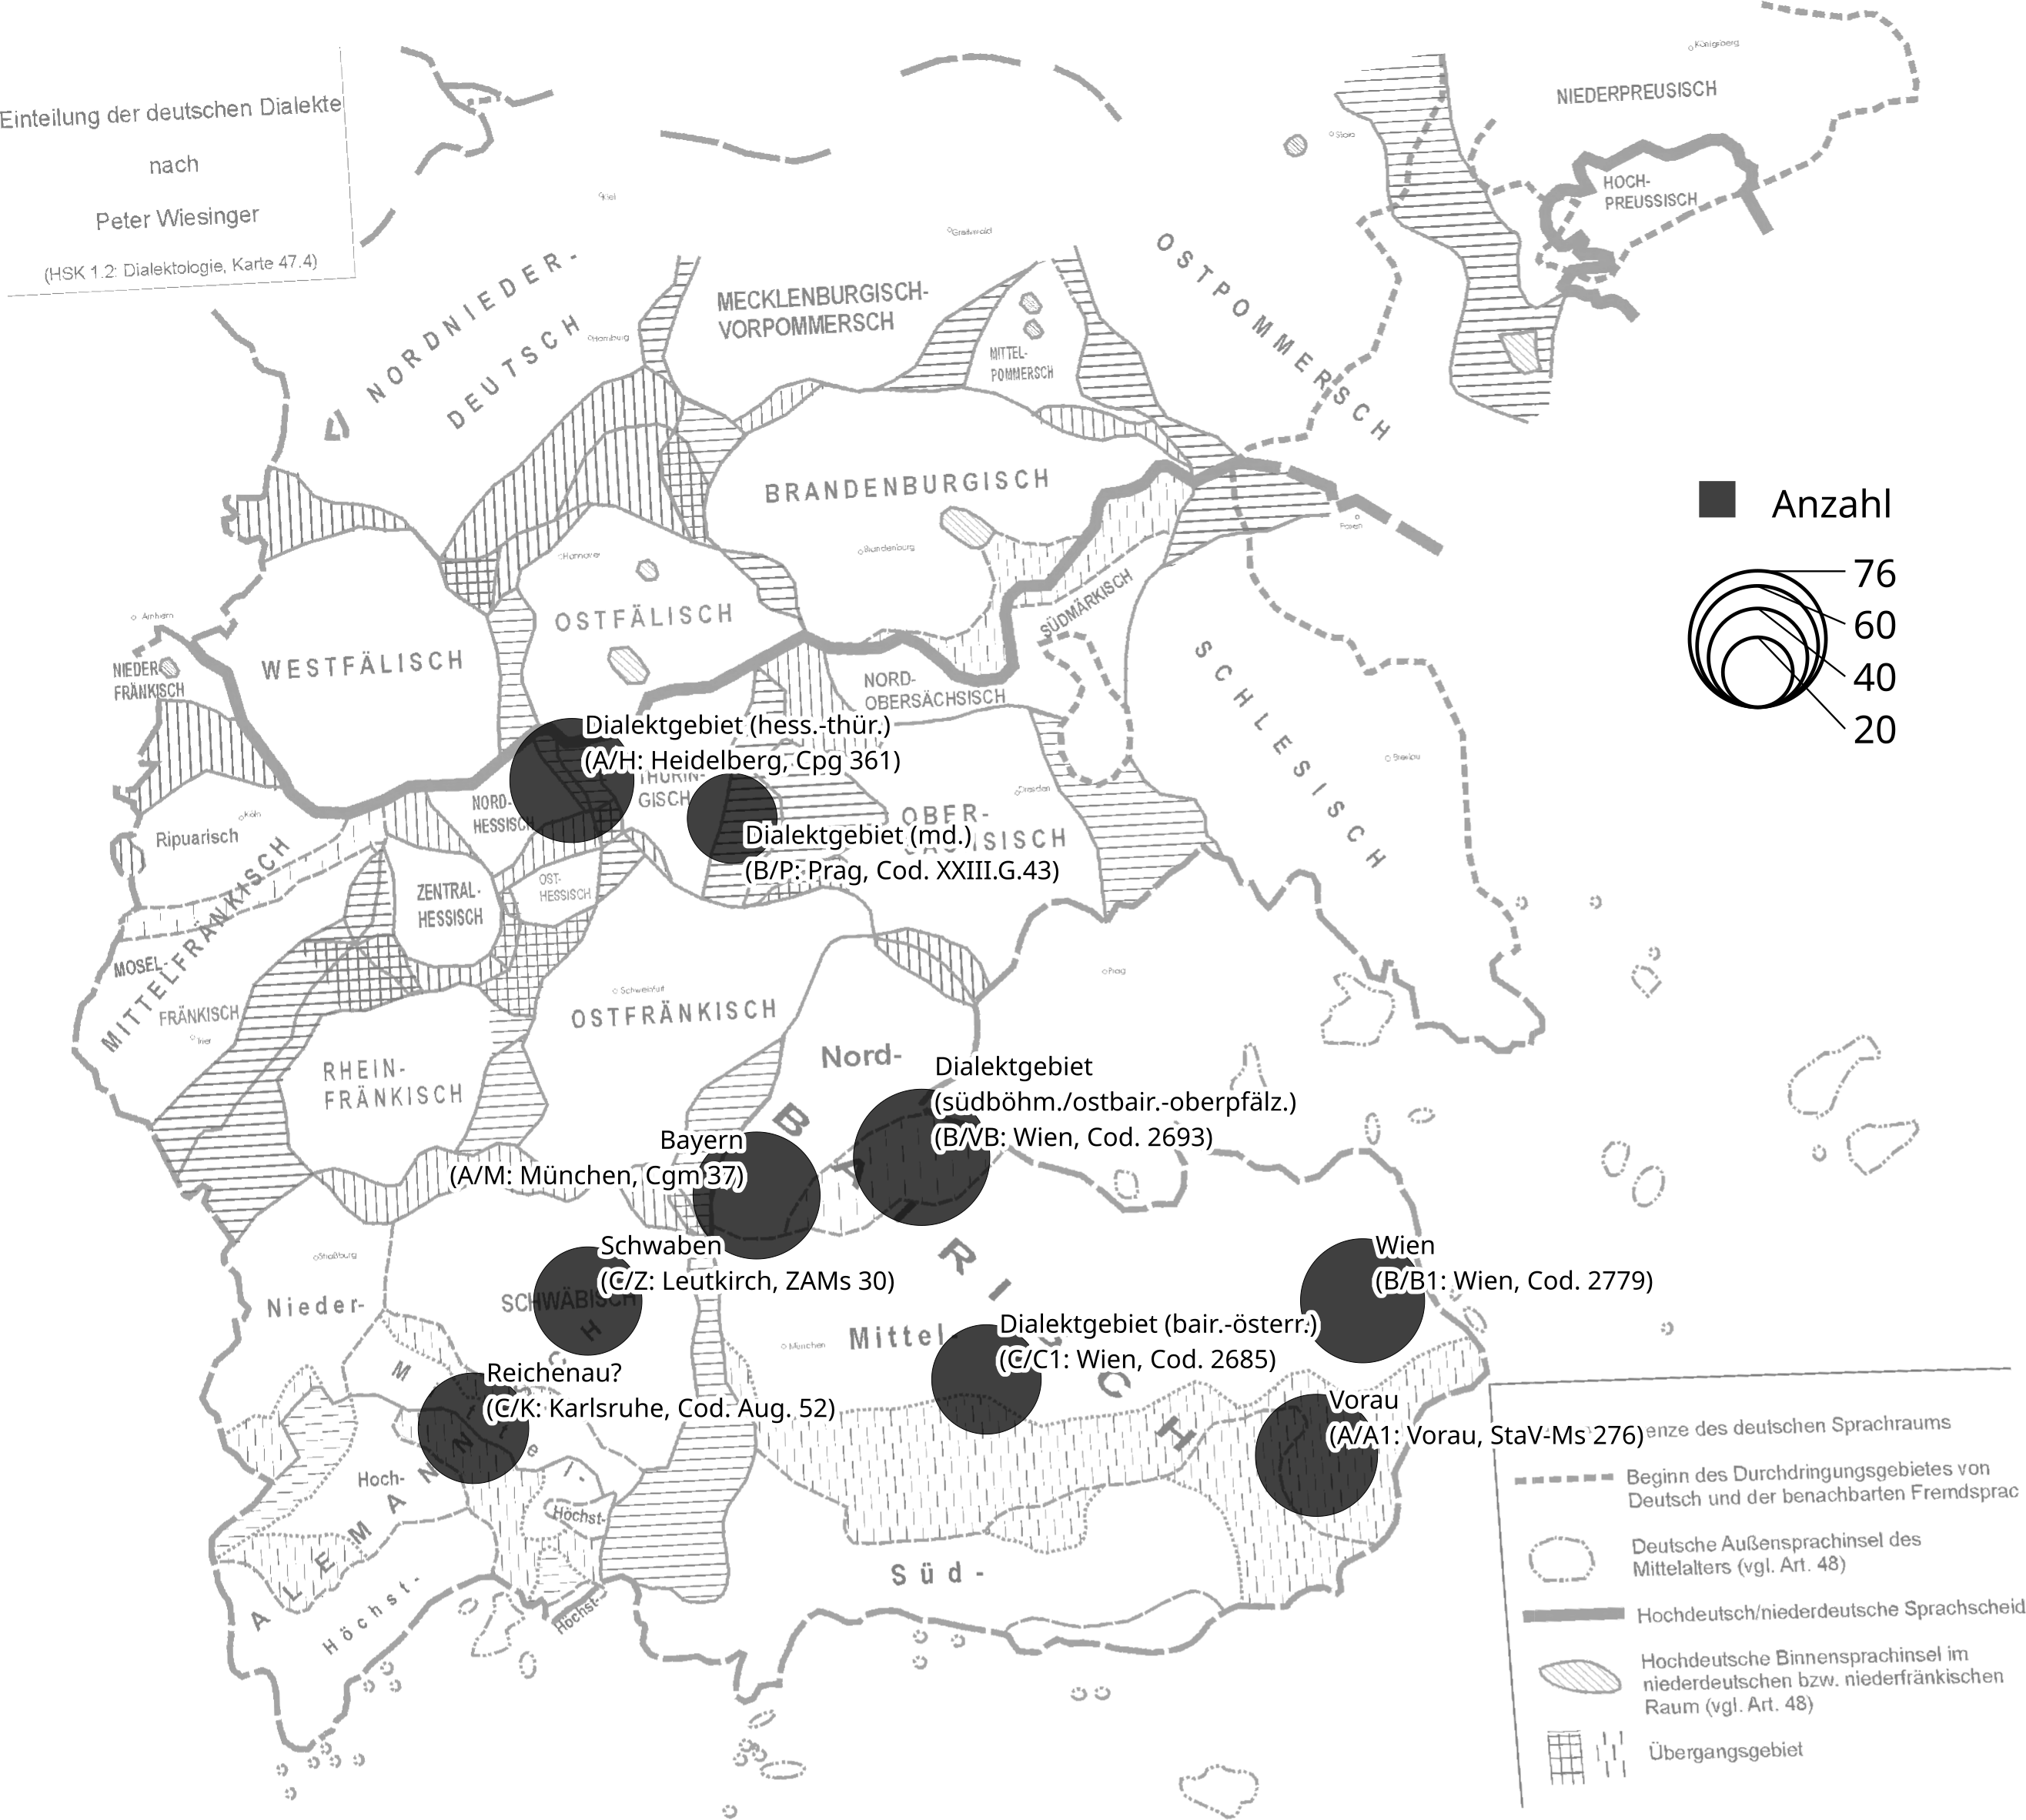
\includegraphics[
	width=\textwidth,
]{./figures/2022-03-07_belege_gebiet.png}
\caption%
	{Anzahl der Belege für mhd.\il{Mittelhochdeutsch} \norm{bėide} pro
	Sprachlandschaft und Handschrift\nocite{wiesinger1983:rede}}
\label{fig:kartebelegzahl}
\end{figure}

Im Regelfall ist bei mittelalterlichen Handschriften keine genaue Einordnung in
Zeit und Raum möglich, da diese -- im Unterschied zu Urkunden -- oft keine
derartigen Selbstauskünfte bieten
\autocites[1309--1310]{wegera2000}[117--121]{bein2011}. Insofern sind bei
den Handschriften C1, H, M, P und VB nur weitläufige Regionen als
(dialekt-)geografische Bezugsgröße angegeben. Die Platzierung der
Handschriften auf der Karte folgt weitestgehend den Angaben des \citetitle{hsc}
\nosh\autocite{hsc} sowie den größtenteils deckungsgleichen Angaben in
\citet{kcdigital} und \citet{wolf:kckat}. Aufgrund der fehlenden Möglichkeit
einer genauen Ortszuweisung in den meisten Fällen haben die markierten Punkte
also lediglich Näherungscharakter und beanspruchen keinesfalls eine geografisch
exakte Festlegung auf den jeweiligen Kartenpunkt.

Darüber hinaus merkt \citet{klein1988} zur Handschrift H an, diese
Handschrift möge \textquote{zwar in Hessen entstanden sein},%
%
	\footnote{Der Terminus \q{Hessen} ist aufgrund der Geschichte des
	Bundeslandes ungenau. Dem Textzusammenhang nach wird wohl die
	Sprachlandschaft gemeint sein, die nicht deckungsgleich mit dem Territorium
	des modernen Bundeslandes ist \autocite[vgl.~z.\,B.][853]{wiesinger1983}.}
%
aber \blockcquote[118]{klein1988}{im
thüringisch\il{Thüringisch}-hessischen\il{Hessisch} Schreibdialekt geschrieben
und zeugt somit nicht für eine rheinische, sondern für eine
thüringisch\il{Thüringisch}-hessische\il{Hessisch}
\q{Kaiserchronik}\nocite{schroeder1895}-Rezeption}. \citet{kcdigital} und
\citet[23]{wolf:kckat} geben mit \citet[237--238]{millerzimmermann2007}
vorsichtig \q{Hessen (Mainz?)} als Entstehungsort an.
\phantomsection%
\label{phsec:vbherkunft}%
Darüber hinaus beobachtet \citeauthor{schneider1987} abweichend von den Angaben
im \citetitle{hsc} und \citet{kcdigital}, dass der Text der Handschrift VB
regelmäßig die eher für das Mitteldeutsche\il{Mitteldeutsch} typische Kennform
\norm{quam} `kam' neben bairischem\il{Bairisch} \norm{chom}
enthält. Obwohl sie dem Schreiber Bemühungen zur Vermeidung von Dialektismen
attestiert, erwägt sie als Entstehungsort den südböhmischen\il{Böhmisch} oder
ostbairisch\il{Bairisch}-oberpfälzischen\il{Oberpfälzisch} Raum
\autocite[226]{schneider1987}.

Neben der räumlichen Dimension spielt bei sprachhistorischen Untersuchungen
auch der zeitliche Bezug eine Rolle. Textzeugen der \KC{} finden sich vom
letzten Viertel des 12.~Jahrhunderts (A1) bis ins späte
16.~Jahrhundert (T), wobei das Gros ins 13./14.~Jahrhundert fällt.
Die in der vorliegenden Untersuchung berücksichtigten Handschriften der
\KC{} entstanden zwischen dem letzten Viertel des 12.~Jahrhunderts und dem
Ende des 15.~Jahrhunderts, wie in \figref{fig:zeitstrahl} gezeigt. Die für die
Auswertung relevanten Textzeugen verteilen sich -- neben A1 aus dem
12.~Jahrhundert -- auf die beiden Jahrhundertviertel um 1300 und stehen damit
zeitlich den Urkunden des \CAO{} nahe.

\begin{figure}[p]
\centering
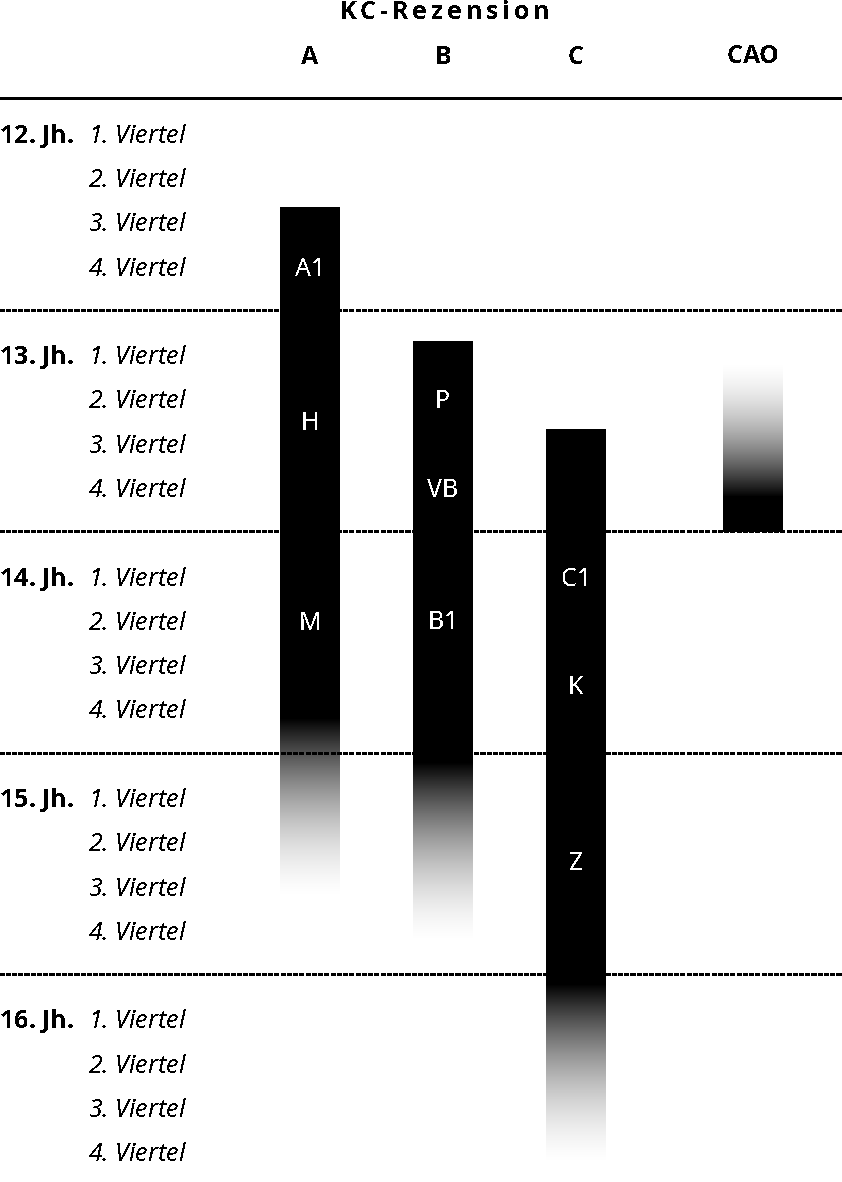
\includegraphics[
	height=.75\textheight,
]{./figures/ueberlieferungszeitraeume.pdf}
\caption{Zeitliche Verteilung der untersuchten Handschriften und Urkunden}
\label{fig:zeitstrahl}
\end{figure}

\section{Targets nach Personenmerkmalen des Controllers}
\label{sec:kctargpers}

\subsection{Nominale Controller}

Wie bei der Belegsammlung zum \CAO{} fällt die Belegmenge für den
direkten Bezug von \norm{bėide} auf zwei nominale Controller im ausgewerteten
\KC{}-Material gering aus. Für den hier untersuchten syntaktischen Kontext
liegen zwei Belege vor; zusammen mit der Kombination von Substantiv und
Pronomen sind es vier. Bei den zum Vergleich gesammelten Belegen zur direkten
Abhängigkeit von einzelnen Controllern im Plural finden sich dagegen 19
Beispiele.

\subsubsection{Kombinierte nominale Controller}
\label{subsubsec:conomctrlpers}

Das Beispiel in \REF{ex:beid2subst} und das Schema in \figref{fig:beid2subst}
verdeutlichen den syntaktischen Kontext, der im Folgenden zu untersuchen sein
wird. Der Quantor \norm{bėide} bezieht sich als Target direkt auf zwei
Controller, \lit{Willehalm} und \lit{Dietreich}, ohne dass eine Pronominalform
dazwischen steht.

\begin{exe}
\protectedex{%
\ex \label{ex:beid2subst}
	\gll Willehalm vnd Dietreich. \\
		Willehalm[\textsc{nom.sg.\MascM}] und Dietrich[\textsc{nom.sg.\MascM}] \\
\sn \gll wurden baíde da erſlagen. \\
		wurden beide-\textsc{nom.pl.\MascM.st} da erschlagen \\
	\trans `Willehalm und Dietrich wurden beide dort erschlagen.'
			(%
				C1:~83vb,36--37%
			)%
}
\end{exe}

\begin{figure}
\begin{tikzpicture}[baseline=(1a_lb.base)]
	\node at (0,2)  (1a)    {\lit{Willehalm}};
	\node           (1a_box)[draw,rectangle,fit=(1a)] {};
	\node           (1a_lb) [above=.5ex of 1a_box, mynodefont]
	                        {controller 1};

	\node at (0,0)  (1b)    {\lit{Dietreich}};
	\node           (1b_box)[draw,rectangle,fit=(1b)] {};
	\node           (1b_lb) [above=.5ex of 1b_box, mynodefont]
	                        {controller 2};

	\node at (3,1) (2)      {\lit{baíde}};
	\draw (2) node (2_box)  [draw,rectangle,fit=(2)] {};
	\node (2_lb)   [above=.5ex of 2_box, mynodefont] {target};

	\draw [-latex] (1a_box) to [out=east, in=west] (2_box);
	\draw [-latex] (1b_box) to [out=east, in=west] (2_box);
\end{tikzpicture}
\caption{Direkter Bezug von \norm{bėide} auf zwei Controller}
\label{fig:beid2subst}
\end{figure}

Die erwähnten vier Belege mit einem \norm{bėide}-Target, das sich direkt auf
zwei Substantive bezieht, verteilen sich auf nur drei verschiedene
Parallelstellen. Die Menge an Kombinationen von Personenmerkmalen wird dadurch
stark reduziert. \tabref{tab:koordnomctrl} gibt eine Übersicht über die Zahl der
Belege für den jeweiligen Flexionstyp und die zugehörige Kombination der
Personenmerkmale der Controller im hier besprochenen syntaktischen Kontext.

\begin{table}
\centering
\caption{Flexion nach Personenmerkmalen der kombinierten nominalen Controller}
\begin{tabular}{
	>{\scshape}l >{\scshape}l
	r r
	r
}
\lsptoprule
\normalfont Controller 1
	& \normalfont Controller 2
	& \norm{bėide}
	& \norm{bėidiu}
	& Summe
	\\

\midrule

3sg.\MascM & 3sg.\MascM &  2 &  1  &  3 \\
3sg.\FemF  & 2sg\subM   &    &  1  &  1 \\

\midrule

\mc{2}{l}{Summe}          &  2 &  2  &  4 \\

\lspbottomrule
\end{tabular}
\label{tab:koordnomctrl}
\end{table}

Von den drei Belegen zur Kombination zweier maskulin-männlicher Referenten sind
zwei derselben Parallelstelle zugehörig: Der Beleg in \REF{ex:dietwill_2}
wurde eingangs zitiert, er sei hier noch einmal im Kontext seiner
Parallelstelle in \REF{ex:dietwill_3} wiedergegeben. Wie erwartet zeigt der
Quantor für diese Merkmalskombination die Form \norm{bėide} in allen Fällen.
Zur dritten Stelle mit \norm{bėidiu} siehe \REF{ex:babstimbaideu}.

\begin{exe}
\ex \label{ex:dietwill} % 203
	\begin{xlist}
	\ex \label{ex:dietwill_2}
		\gll Willehalm vnd Dietreich. \\
			Willehalm[\textsc{nom.sg.\MascM}] und Dietrich[\textsc{nom.sg.\MascM}] \\
	\sn \gll wurden baíde da erſlagen. \\
			wurden beide-\textsc{nom.pl.\MascM.st} da erschlagen \\
		\trans `Willehalm und Dietrich wurden beide dort erschlagen.'
			(%
				C1:~83vb,36--37%
			)

	\ex \label{ex:dietwill_3}
		\gll Wilhalm vnd dietrich \\
			Willehalm[\textsc{nom.sg.\MascM}] und Dietrich[\textsc{nom.sg.\MascM}] \\
	\sn \gll Wurden baide do erſlagen \\
			wurden beide-\textsc{nom.pl.\MascM.st} da erschlagen \\
		\trans `Willehalm und Dietrich wurden beide dort erschlagen.'
			(%
				K:~95vb,12--13%
			)
	\end{xlist}
\end{exe}

Beispiele für die Kombination von maskulin-männlichen und feminin-weib\-lichen
Substantiven ($\MascM+\FemF$, $\FemF+\MascM$) liegen im hier untersuchten
Kontext zumindest formal keine vor. Es gibt allerdings einen Einzelbeleg für
die Kombination von weiblicher und männlicher Referenz bei Substantiv und
Personal\-pronomen, der in \REF{ex:mutterdu} wiedergegeben wird.

\begin{exe}
\ex\label{ex:mutterdu}
	\gll Zvͦ dem chûnig ſprach er ſan \\
		zu dem König[\textsc{dat.sg.\MascM}] sprach er sodann \\
	\textelp{}
\sn \gll Dein muͦter vnd dv \\
		dein Mutter[\textsc{nom.sg.\FemF}] und \textsc{2sg\subM.nom} \\
\sn \gll Schv̂ln beideu chv̂men {dar zvͦ} \\
		sollen beide-\textsc{nom.pl.\NeutMF.st} kommen dahin \\
	\trans `Zum König sprach er sodann: \enquote{\textelp{} Deine
		Mutter und du sollt beide dahin kommen.}'
		(%
			B1:~23rc,5--14%
		)
\end{exe}

Hier verbirgt sich hinter dem \lit{dv} `du' trotz fehlender
Genusmarkierung beim Pronomen der 2.\ Pers.\ Sg.\ ein männlicher Referent,
nämlich der \lit{chûnig} `König', der direkt angesprochen wird. Der Beleg
passt damit in das Bild, das schon die Auswertung der Urkunden ergeben hat.
Auch bei Pro\-nomina ohne Genusmarkierung tritt aufgrund der referenzierten Personenmerkmale bei kombiniertem Bezug die
neutrale Form auf.

\phantomsection
\label{phsec:babstimbaideu}
Der Beleg in \REF{ex:babstimbaideu} mit \norm{bėidiu} in Bezug auf zwei
männliche Referenten wurde bereits erwähnt. Die Passage wurde hier so
interpretiert, dass sich \lit{ím} `ihm' auf \lit{Karle} `Karl (der
Große)' bezieht, also nicht auf \lit{wideme} `Dotierungen, Stiftungen'
\autocite[vgl. zur  Definition][s.\,v.~\fw{wideme}]{lexer:mhdhwb} und
\lit{zehende} `Zehnten'. Letzteres Wortpaar steht im Genitiv Plural
\autocite[vgl.][341]{paul2007}, sodass die erwartete Kongruenzform des
Quantors regelmäßig \norm{bėider(e)} `beider' lauten müsste. Andere Belege
mit \norm{bėidiu} als Genitivform wurden weder für diese Handschrift noch für
die anderen exzerpiert.%
%
	\footnote{In Bezug auf den Text der Edition von
	\citet{schroeder1895} übersetzt \citet[249]{mayer1874}:
	\blockquote{Als König Karl dann zu Gericht saß, trat der Pabst vor ihn hin
	und klagte, daß die Rechte, welche seinen Vorfahren seien verliehen worden,
	ihm von den Römern entrissen wurden, so seien ihm namentlich Zehenten und
	Widdume genommen}; vgl. auch \citet[83]{weis2022}.}

\begin{exe}
\ex\label{ex:babstimbaideu}
	\gll Karle an daz gerichte ſaz \\
		Karl[\textsc{nom.sg.\MascM}] an das Gericht saß \\
\sn \gll Der babſt klegt ím daz \\
		der Papst[\textsc{nom.sg.\MascM}] klagte \textsc{3sg.\MascM.dat} dass \\
\sn \gll Der wideme vnd der zehende gar \\
		der Dotierungen und der Zehnten gar \\
\sn \gll Waͤren baidu̍ worden bar \\
		wären beide-\textsc{nom.pl.\NeutM.st} geworden ledig \\
\sn \gll Von ſínen vorvarn \\
		von seinen Vorfahren \\
	\trans `Karl setzte sich zu Gericht. Der Papst klagte ihm, dass
		\textins{sie} beide an Dotierungen und gar an Zehnten ledig geworden
		wären durch seine Vorfahren.'
		(%
			K:~85vb,22--24; vgl. abweichend
			\KC:~V.~14383--14385;
			\cite[341]{schroeder1895}%
		)
\end{exe}

Erfahrungsgemäß sollte man vorsichtig sein, Erwartungen an die Grammatik
mittelhochdeutscher\il{Mittelhochdeutsch} Texte zu stellen. Jedoch ist die Form
\lit{beider} in K ansonsten die für den Gen.\ Pl.\ regelmäßig belegte, wie die
Beispiele in \REF{ex:k_beider} zeigen, sodass davon ausgegangen werden kann,
dass sich \lit{baidiu} an dieser Stelle tatsächlich auf Karl und den Papst
bezieht.

\begin{exe}
\ex \label{ex:k_beider}
	\begin{xlist}
	\ex \label{ex:k_beider_1}
		\gll V̍nſer baider kínt \\
			unser beide-\textsc{gen.pl.st} Kind \\
	\sn \gll Bevilch ich allen die hie ſínt \\
			befehle ich allen die hier sind \\
		\trans `Unser beider Kind befehle ich allen an, die hier sind.'
			(%
				K:~9rb,25--26; vgl.
				C1:~8vb,27--28;
				% VC:~6va,13--14;
				Z:~31va,3--4; abweichend
				A1:~7va,3--4;
				H:~9va,42--43;
				P:~15va,14--15;
				\KC:~V.~1639;
				\cite[111]{schroeder1895}%
			)

	\ex \label{ex:k_beider_2}
		\gll In Rome bi ír baider zít \\
			in Rom bei ihr beide-\textsc{gen.pl.st} Zeit \\
	\sn \gll Huͦb ſich vrlu̍g vnd ſtrit \\
			hob sich Krieg und Kampf \\
		\trans `Zu ihrer beider Zeit erhoben sich in Rom Kampf und Krieg.'
			(%
				K:~28vb,36--37; vgl.
				% VC:~17va,31--32;
				Z:~93va,26--94ra,1; abweichend
				B1:~14va,49--50;
				VB:~24ra,30--31;
				P:~42ra,17--18;
				A1:~20vb,9--10;
				M:~36rb,6--7;
				H:~28rb,39--40;
				\KC:~V.~4837--4838;
				\cite[170]{schroeder1895}%
			)

	\ex \label{ex:k_beider_3}
		\gll Daz waz ír baider vngewín \\
			Das war ihr beide-\textsc{gen.pl.st} Verlust \\
		\trans `Das war ihr beider Verlust.'
			(%
				K:~103vb,27; vgl.
				C1:~91va,10;
				% VC:~60va,34;
				Z:~352ra,6;
				\KC:~V.~208;
				\cite[83]{schroeder1895}%
			)
	\end{xlist}
\end{exe}

\subsubsection{Einfache nominale Plural-Controller}
\label{subsubsec:nomctrlpers}

In diesem Abschnitt werden zum Vergleich Belege wie der in
\REF{ex:beidplsubst} angeführte und in \figref{fig:beidplsubst} illustrierte
diskutiert. Das Target \lit{bêde} `beide' ist hier ebenfalls unmittelbar auf
seinen Controller bezogen. Im Vergleich zum vorigen Abschnitt handelt es sich
beim Controller jedoch nicht um die Kombination von Substantiven, sondern nur
um ein einzelnes Substantiv, das im Plural steht.

\begin{exe}
\ex \label{ex:beidplsubst}
	\gll die {gotes boten} bêde \\
		 die Gottesboten[\textsc{nom.pl.\MascM}] beide-\textsc{nom.pl.\MascM.st} \\
	\trans `die beiden Gottesboten'
		(%
			\KC:~V.~7845;
			\cite[225]{schroeder1895}%
		)
\end{exe}

\begin{figure}
\begin{tikzpicture}[baseline=(1_lb.base)]
	\node (1)      [align=center]
	               {\lit{gotes boten}};
	\node (1_box)  [draw,rectangle,fit=(1)] {};
	\node (1_lb)   [above=.5ex of 1_box, mynodefont]{controller};

	\node (2)      [right=4em of 1_box, align=center]
	               {\lit{bêde}};
	\draw (2) node (2_box1) [draw,rectangle,fit=(2)] {};
	\node (2_lb1)  [above=.5ex of 2_box1, mynodefont] {target};

	\draw [-latex] (1_box) to (2_box1);
\end{tikzpicture}
\caption{Direkter Bezug eines Targets auf einen einzelnen Controller}
\label{fig:beidplsubst}
\end{figure}

Kontexte, in denen \norm{bėide} in einer direkten Kongruenzbeziehung mit einem
einzigen Substantiv im Plural steht, sind auch in der \KC{} im Vergleich
zu Kontexten mit kombinierter Referenz zahlreicher vorhanden.
\tabref{tab:simpnomctrla} zeigt ihre Verteilung nach Personenmerkmalen und
Flexionstyp.

\begin{table}
\centering
\caption{Flexion nach Personenmerkmalen der einfachen nominalen Controller}
\begin{tabular}{>{\scshape}l r r r}
\lsptoprule
\normalfont Controller
	& \norm{bėid(e)}
	& \norm{bėidiu}
	& Summe
	\\

\midrule

\MascM  & 11 &  2 & 13 \\
\NeutM  &    &  1 &  1 \\
\NeutA  &    &  1 &  1 \\

\midrule

\FemI   &  1 &    &  1 \\

\midrule

\normalfont Summe & 12 &  4 & 16 \\

\lspbottomrule
\end{tabular}
\label{tab:simpnomctrla}
\end{table}

Mit elf Belegen zu fünf Stellen verteilen sich die meisten
\norm{bėid(e)}-Formen mit maskulin-männlichem Bezug wie nach formalen Kriterien
erwartet \autocite[vgl.][182]{ksw2}. Interessant sind in diesem Kontext die
Abweichungen, das heißt, die zwei Belege für \norm{bėidiu} mit
maskulin-männlichem Bezug. Diese werden in \REF{ex:richtherriu} wiedergegeben.
Starke Adjektive zeigen in B1 ansonsten \norm{-iu} im Plural
regel\-mäßig nur bei den Neutra; Maskulina und Feminina sind dagegen stets
endungslos (vgl.~\tabref{tab:kcadjdeclovw}).

\begin{exe}
\ex \label{ex:richtherriu}
	\begin{xlist}
	\ex \gll Die rihtær ſprachen beideu {dar zuͦ} \\
			die Richter[\textsc{nom.pl.\MascM}] sprachen beide-\textsc{nom.pl.\NeutM.st}
			dazu \\
		\trans `Die Richter äußerten sich beide dazu'
			(%
				B1:~28ra,8; vgl.~abweichend
				\KC:~V.~10090;
				\cite[267]{schroeder1895}% 1140 mit Parallelstelle in H
			)
		\label{ex:richtherriu_1}

	\ex \gll Die herren baten ir ſa \\
			Die Herren[\textsc{nom.pl.\MascM}] baten ihr alsbald \\
	\sn \gll Beideu beſvnder \\
			beide-\textsc{nom.pl.\NeutM.st} einzeln \\
		\trans `Die Herren hielten alsbald jeweils beide um ihre Hand an.'
			(%
				B1:~31va,48--49; vgl.
				\KC:~V.~11385--11386;
				\cite[289]{schroeder1895}% 1112x
			)
		\label{ex:richtherriu_2}
	\end{xlist}
\end{exe}

\phantomsection
\label{phsec:baideuwarn}
Der Beleg zu \norm{bėidiu} bei einem Neutrum mit männlichem Bezug in
\REF{ex:baideuwarn}, ein Parallelbeleg zu dem in \REF{ex:babstimbaideu}
zitierten, enthält formale Kongruenz. Das Lexem \lit{warn} `Kinder' zu
mittelhochdeutsch\il{Mittelhochdeutsch} \norm{barn} `Kind, Sohn; Jüngling, Held
(?)' \autocites[s.\,v.\fw{barn}]{mwb1}[vgl.~auch][53]{kroonen2013} bezieht sich
hier metaphorisch auf Karl den Großen und Papst Leo~III., die vom
Kaiserchronisten als Brüder dargestellt werden (V.~14370;
\cites[341]{schroeder1895}[vgl.][83]{weis2022}). Obwohl sich \lit{warn} also
auf zwei erwachsene Männer bezieht, was die Wahrscheinlichkeit für semantische
Kongruenz erhöht (siehe \sectref{sec:gendsex}), zeigt der Quantor in formaler
Übereinstimmung mit seinem Controller die neutrale Form.

\begin{exe}
\protectedex{%
\ex \label{ex:baideuwarn}
	\gll der wídem vnd der zehent gar. \\
		der Dotierungen und der Zehnten gar \\
\sn \gll wærn baidev warn bar. \\ % 1123
		wären beide-\textsc{nom.pl.\NeutM.st} Kinder[\textsc{nom.pl.\NeutM}] ledig \\
	\trans `an Dotierungen und Zehnten wären beide Kinder ledig'
		(%
			C1:~75rb,3--4; vgl.~abweichend
			K:~85vb,24;
			\KC:~V.~14384--14385;
			\cite[341]{schroeder1895}%
		)%
}
\end{exe}

Auch der Quantor in \REF{ex:beideuher} dekliniert nach dem neutralen Genus
gemäß formaler Kongruenz innerhalb der Nominalphrase (NP). In
\tabref{tab:simpnomctrla} wurde dieser Beleg mit \SA\ gekennzeichnet, da
\lit{her} `Heer' bei der Annotation als Committee Noun
\autocite[211--213]{corbett2006} aufgefasst wurde: Der Begriff, obwohl formal
im Singular, bezieht sich in seiner Semantik auf eine Gruppe von Menschen. In
jedem Fall zeigt sich nicht das Fehlen von overter Flexion, die ansonsten in
der Stichprobe zu B1 für den starken Nom./Akk.~Pl.~M./F. belegt ist.

\begin{exe}
\ex \label{ex:beideuher}
	\gll Der wær herre ûber beideu her \\
		der wäre Herr über beide-\textsc{acc.pl.\NeutA.st} Heer[\textsc{acc.pl.\NeutA}] \\
	\trans `Der wäre Herr über beide Heere'
		(%
			B1:~31rc,3; zu
			\KC:~V.~11272\,ff.;
			\cite[287]{schroeder1895}% 1110
		)
\end{exe}

Der Beleg für ein unbelebtes Femininum hat die Form \lit{baide}, insofern auch
hier der Quantor innerhalb der NP formale Kongruenz zeigt
\REF{ex:uozehende_2}, obwohl es sich um Körperteile handelt und damit um
etwas, von dem auszugehen ist, dass es eine mittlere Position zwischen den
Polen belebt und unbelebt einnimmt (vgl.~\sectref{sec:gendsex} zur Annotation von
Genus bei Inanimata).

\begin{exe}
	\ex \gll Si wand ír baide hênde \\
			sie wand ihr beide-\textsc{acc.pl.\FemI.st} Hand-\textsc{acc.pl.\FemI} \\
		\trans `Sie wand ihre beiden Hände.'
			(%
				K:~6rb,19; vgl.
				\KC:~V.~913;
				\cite[98]{schroeder1895}%
			)
		\label{ex:uozehende_2}
\end{exe}

\subsubsection{Zusammenfassung}

Die Belegstellen zum kombinierten direkten Bezug von \mbox{\norm{bėide}} auf
zwei Substantive fallen nicht aus dem Rahmen bisheriger Ergebnisse, wenn es
auch die geringe Belegzahl unmöglich macht, generelle Aussagen zu treffen. In
beiden Fällen zeigte sich die Form \norm{bėide} mit Bezug auf maskuline und
feminine Referenten. Im Fall der Kongruenz eines Quantors mit einem einzelnen
Substantiv im Plural wiesen die Targets innerhalb der NP ebenfalls formale
Kongruenz auf, doch liegen zwei Belege für neutrales \norm{bėidiu} bei
eindeutig maskulin-männlichem Bezug vor.

\subsection{Anaphorische Controller}

Mit 19 Stellen liegt der größere Teil des Belegmaterials zur \KC{} für die
Kongruenzrelation zwischen \norm{bėide} in indirekter Abhängigkeit von zwei
nominalen Controllern vor. Die Kombination von Substantiv und einem Pronomen
der ersten oder zweiten Person als Diskurs\-anker wird hier mitgezählt.
Textstellen mit indirektem Bezug zwischen Quantor und einzelnem Substantiv im
Plural sind neun vorhanden.

\subsubsection{Indirekter Bezug auf kombinierte nominale Controller}
\label{subsubssec:iconomctrlpers}

Hier soll zunächst der Kongruenzbezug zwischen kombinierten Controllern und
Quantor mit einem Pronomen als Verbindungsglied anhand der gesammelten Belege
untersucht werden. Das Verhältnis zwischen Kongruenzcontrollern und Target wird
in \REF{ex:beidanactrl} und \figref{fig:beidanactrl} illustriert.%
%
	\footnote{Auch für die \KC{} gilt, dass das Personalpronomen der
		3.~Pers.\ Pl.\ Nom./Akk. in der Regel zu \norm{si} ausgeglichen
		erscheint, also keine Differenzierung zwischen maskulin-femininem
		\norm{sie} und neutralem \norm{siu} nachzuvollziehen ist, vergleiche
		\citet[213--214]{paul2007} und \citet[369, 390--397]{ksw2} sowie die
		Teiluntersuchung zur Form des Pronomens in
		\sectref{subsubsec:monoflexionkc}.}

\begin{exe}
\ex\label{ex:beidanactrl}
	\gll Si nâmen di muoter mit dem sun, \\
		sie nahmen die Mutter[\textsc{acc.sg.\FemF}] mit dem Sohn[\textsc{dat.sg.\MascM}] \\
\sn \gll si viengen si bî dem hâre, \\
		sie fingen \textsc{3pl\subMF.acc} an dem Haare \\
\sn \gll si vuorten si baide zewâre \\
		sie führten \textsc{3pl\subMF.acc} beide-\textsc{acc.pl.m+f\subMF.st}
			wirklich \\
\sn \gll vur die burch an daz velt \\
		vor die Stadt an das Ebene \\
	\trans `Sie nahmen die Mutter mit dem Sohn. Sie fingen sie an den
		Haaren. Ja, sie führten sie beide vor die Stadt zu der Ebene.'
		(%
			KC:~V.~14269--14272;
			\cite[339]{schroeder1895}%
		)
\end{exe}

\begin{figure}
\begin{tikzpicture}[baseline=(1a_lb.base)]
	\node at (0,2)  (1a)    [gray]
	                        {\lit{muoter}};
	\node           (1a_box)[draw,gray,rectangle,fit=(1a)] {};
	\node           (1a_lb) [above=.5ex of 1a_box, gray, mynodefont]
	                        {controller 1};

	\node at (0,0)  (1b)    [gray]
	                        {\lit{sun}};
	\node           (1b_box)[draw,gray,rectangle,fit=(1b)] {};
	\node           (1b_lb) [above=.5ex of 1b_box, gray, mynodefont]
	                        {controller 2};    

	\node at (3,1) (2)      {\lit{si}};
	\draw (2) node (2_box1) [
	                    draw,
	                    gray,
	                    minimum height=3em,
	                    minimum width=3em,
	                    xshift=-.5ex,
	                    yshift=+.5ex,
	                    rectangle
	                ] {};
	\draw (2) node (2_box2) [
	                    draw,
	                    minimum height=3em,
	                    minimum width=3em,
	                    xshift=+.5ex,
	                    yshift=-.5ex,
	                    rectangle
	                ] {};
	\node           (2_lb1) [above=.5ex of 2_box1, gray, mynodefont]
	                        {target};
	\node           (2_lb2) [below=.5ex of 2_box2, mynodefont]
	                        {controller};

	\node at (6,1)  (3)      {\lit{baide}};
	\node           (3_box)  [draw,rectangle,fit=(3)] {};
	\node           (3_lb)   [above=.5ex of 3_box, mynodefont]
	                        {target};

	\draw [-latex,gray] (1a_box) to [out=east, in=west] (2_box1);
	\draw [-latex,gray] (1b_box) to [out=east, in=west] (2_box1);
	\draw [latex-]      (3_box)  to [yshift=1.5ex]      (2_box2);
\end{tikzpicture}
\caption{Indirekter Bezug eines Targets auf zwei \q{Erstcontroller} über ein Personalpronomen}
\label{fig:beidanactrl}
\end{figure}

Auch wenn es sich bei \lit{muoter mit dem sun} `Mutter mit dem Sohn' nicht
strikt um eine syntaktische Koordination vom Typ \q{X \fw{und}
Y} handelt (vgl.~\sectref{sec:erwkonjbegr} zur \q{erweiterten}
Koordination), werden \lit{muoter} `Mutter' und \lit{sun} `Sohn'
durch \lit{si} `sie' kombiniert zusammengefasst. Der Quantor \lit{baide}
modifiziert dieses \lit{si} und kongruiert mit ihm. Der Quantor kongruiert
damit direkt mit dem Personalpronomen \lit{si} und indirekt mit \lit{muoter}
und \lit{sun}.

\tabref{tab:kcsimprefctrl} gibt die Belegverteilung in der \KC{} für die in
\REF{ex:beidanactrl} exemplarisch ausgeführte Kongruenzrelation wieder,
wobei auch hier nur Handschriften berück\-sichtigt wurden, die beide
Kongruenzformen aufweisen (effektiv: B1 und VB; vgl.~auch
\sectref{sec:adjdeclkc} zur Adjektivdeklination in \KC{}-Handschriften).

\begin{table}
\centering
\caption{Flexion nach Personenmerkmalen der anaphorischen Controller
(kombinierter Bezug)}
\begin{tabular}{
	>{\scshape}l @{$~+~$} >{\scshape}l
    r r
    r
}
\lsptoprule
\mc{2}{c}{Controller}
    & \norm{bėid(e)}
    & \norm{bėidiu}
    & Summe
    \\

\midrule

% Controller              | e  | iu | Σ
3sg.\MascM & 3sg.\MascM & 11 &  1 & 12 \\

\midrule

1sg\subF & 2sg\subX     &  1 &  1 &  2 \\
2sg\subM & 1sg\subF     &    &  1 &  1 \\
2sg\subM & 3sg.\FemF    &    &  1 &  1 \\

\midrule

\mc{2}{l}{Summe}          & 12 &  4 & 16 \\

\lspbottomrule
\end{tabular}
\label{tab:kcsimprefctrl}
\end{table}

In \tabref{tab:kcsimprefctrl} entfällt textbedingt der größte Anteil auf die
Kombination zweier maskulin-männlicher Referenten ($3sg.\MascM +
3sg.\MascM$). Insgesamt weisen 14 von 16 Belegen (zu zwölf Textstellen) die zu
erwartende Flexionsform auf. Bei den zwei übrigen Belegen handelt es sich um
einen Beleg vom Typ \norm{bėide} mit Bezug auf zwei Neutra sowie einen Beleg
für \norm{bėidiu} bei kombinierten Maskulina.

Für die vorliegende Untersuchung am interessantesten ist das Belegpaar zur 1.\
Pers.\ Sg. (weiblich) in Kombination mit einer 2.\ Pers.\ Sg.: An der
betreffenden Stelle spricht ein \norm{wīp} `Frau' zu seinem
\norm{kindelīn} `Kindlein' (V.~910--932; \cite[98]{schroeder1895}). Das
Geschlecht des Kindes ist unbekannt; es muss sich dem Kontext nach um einen
Säugling handeln. Die beiden Belegstellen werden in \REF{ex:wipkindelin}
wiedergegeben.

\begin{exe}
\ex \label{ex:wipkindelin}
	\begin{xlist}
	\ex \label{ex:wipkindelin_1}
		\gll Sit wír nv mvͤzzen verderben \\
			da \textsc{1pl\tsub{\SF/\SX}.nom} nun müssen zugrunde.gehen \\
	\sn \gll Vnd beide von den heiden ſterben \\
			und beide-\textsc{nom.pl.m+f\tsub{\SF/\SX}.st} von den Heiden
				sterben \\
		\trans `Da wir (jetzt) wohl zugrunde gehen werden und beide durch die Heiden sterben.'
			(%
				VB:~5rb,33--34; vgl.~abweichend
				\KC:~V.~931--932;
				\cite[98]{schroeder1895}%
			)
		
	\ex \label{ex:wipkindelin_2}
		\gll Seit wir muͤzzen verderben. \\
			da \textsc{1pl\tsub{\SF/\SX}.nom} müssen zugrunde.gehen \\
	\sn \gll und beideu von den haiden ſterben \\
			und beide-\textsc{nom.pl.n\tsub{\SF/\SX}.st} von den Heiden
				sterben \\
		\trans `Da wir (jetzt) wohl zugrunde gehen werden und beide durch die Heiden sterben.'
			(%
				B1:~4vb,57--58; vgl.~abweichend
				\KC:~V.~931--932;
				\cite[98]{schroeder1895}%
			)
	\end{xlist}
\end{exe}

In der Klassifikation in \tabref{tab:kcadjdeclovw} gehört VB zur
Gruppe 3. Das bedeutet, dass in der Stichprobe zur Adjektiv\-flexion leichte
Variation zwischen \norm{-iu} und \norm{-e} im Plural Neutrum vorliegt, wobei
\norm{-iu} überwiegt. Um einen solchen Fall mag es sich auch hier handeln.
Daneben besteht die Möglichkeit, dass in \REF{ex:wipkindelin_1} der generellen
Belebtheit der Controller wegen die Form \lit{beide} auftritt. Die Form
\lit{beideu} in \REF{ex:wipkindelin_2} passt zum einen zur Kombination von
zwei formalen Neutra, zum anderen als Resolutionsform, insofern weiblich und
\q{unspezifisch} keine Schnittmenge besitzen
(vgl.~\sectref{subsubsec:x+x_dir_anim} zur theoretischen Modellierung der
Kombination von Genusmerkmalen).

Der andere oben genannte Beleg mit \norm{bėidiu} statt regelhaftem \norm{bėide}
bei der Kombination zweier Maskulina wird in \REF{ex:papstkoenig} angeführt.
Die \norm{iu}-Form des Quantors bei kombiniertem männlichen Bezug ist
irregulär. % (vgl.~\sectref{subsec:m+m_anim_beidiu}).

\begin{exe}
\protectedex{%
% Gerade dieses Beispiel bricht nie gut um. Zeilenumbrüche entfernt, "/"
% zwischen Versen eingefügt.
\ex\label{ex:papstkoenig} % 224
	\gll Der papſt vnd der chv̂nich {/} \\
		der Papst[\textsc{nom.sg.\MascM}] und der
		König[\textsc{nom.sg.\MascM}] \\
	\gll Si warn zegot biderb vnd frumic {/} \\
		\textsc{3pl\subM.nom} waren {zu=Gott} brav und tüchtig {} \\
	\gll Zegot ſtuͦnt allr ir geſín {/} \\
		{zu=Gott} stand aller ihr Sinnen \\
	\gll Beideu ſchatz vnd gewín {/} \\
		beide Schatz und Gewinn \\
	\gll Liezzen ſi beideu gelich {/} \\
		ließen \textsc{3pl\subM.nom} beide-\textsc{nom.pl.\NeutM.st} gleich \\
	\trans `Der Papst und der König, sie waren Gott gegenüber brav und
		tüchtig. Auf Gott war all ihr Sinnen gerichtet. Sowohl Schatz als auch
		Gewinn war ihnen beiden gleich.'
		(%
			B1:~17vb,30--34; vgl.~abweichend
			\KC:~V.~6110--6113;
			\cite[202]{schroeder1895}%
		)%
}
\end{exe}

Sowohl bei \lit{ſchatz} `Schatz' als auch bei \lit{gewín} `Gewinn'
handelt es sich um unbelebte Maskulina. Es scheint im Kontext der Stelle
sinnvoller, das neutrale \lit{beideu} in Zeile~34 nicht darauf, sondern auf
\lit{ſi} -- den \lit{papſt} `Papst' und den \lit{chv̂nich} `König' --
zu beziehen. Der Blick in die Parallelstellen in VB und
A1 stützt diese Interpretation, insofern es hier trotz abweichendem
Wortlaut eindeutig um das gottgefällige Handeln von Kaiser Philippus und Papst
Sixtus geht \REF{ex:papstkoenig2}.

\begin{exe}
\ex\label{ex:papstkoenig2}
\begin{xlist}
	\ex \label{ex:papstkoenig2_1}
		\gll Beidiv ſchatz vnd gewín \\
			beide Schatz[\textsc{acc.sg.\MascI}] und Gewinn[\textsc{acc.sg.\MascI}] \\
	\sn \gll Liezzen ſie gelíche. \\
			ließen \textsc{3pl\subM.nom} gleich \\
		\trans `Sowohl Schatz als auch Gewinn war ihnen gleich.'
			(%
				VB:~29vb,38%
			)

	\ex \label{ex:papstkoenig2_2}
		\gll baidiv ſcaz unde gewin. \\
			beide Schatz[\textsc{acc.sg.\MascI}] und Gewinn[\textsc{acc.sg.\MascI}] \\
	\sn \gll liezen ſi in beſlifen. \\
			ließen \textsc{3pl\subM.nom} \textsc{refl.dat.pl\subM} entgehen \\
		\trans `Sowohl Schatz als auch Gewinn ließen sie sich entgehen'
			(%
				A1:~26rb,40--41; vgl.
				H:~36ra,40--41;
				\KC:~V.~6112--6113;
				\cite[202]{schroeder1895}%
			)
\end{xlist}
\end{exe}

Für den kombinierten Bezug auf Personen von eindeutig unterschiedlichem
Geschlecht liegt zumindest ein einziger Beleg vor. Die Kombination von 2.\
Pers. Sg.\ (männlich) und 1.\ Pers.\ Sg.\ (weiblich) wird durch
\norm{bėidiu} aufgenommen, womit Gender Resolution vorliegt: \lit{so wærn wir
baidev verloͤrn} `dann wären wir beide verloren' (C1:~60rb,44--60va,3).

\subsubsection{Indirekter Bezug auf unkombinierte Plural-Controller}
\label{subsubsec:beid2p2snglnkc}

Beim indirekten Bezug zwischen einem einzelnen Substantiv im Plural und
\norm{bėide} als Target wie in \REF{ex:nplsibeide} und \figref{fig:nplsibeide}
liegt in der Stichprobe zur \KC{} keine Variation vor. In allen neun Fällen
sind ausschließlich Formen von \norm{bėid(e)} belegt, davon besitzen alle eine
männlich-maskuline Referenz.

\begin{exe}
\ex \label{ex:nplsibeide}
	\gll do die hêrren pranten \\
			als die Herr-\textsc{nom.pl.\MascM} brannten \\
	\textelp{}
\sn \gll da ze Kastel er si baide begraif \\
			dort zu Kastel er \textsc{3pl\subM.acc}
			beide-\textsc{acc.pl.\MascM.st} ergriff \\
		\trans `Als die Herren brandschatzten \textelp{} Dort in Kastel ergriff
			er sie beide'
			(%
				\KC:~V.~16104--16111;
				\cite[372]{schroeder1895}%
			)
\end{exe}

\begin{figure}
\begin{tikzpicture}[baseline=(2_lb1.base)]
    \node at (0,0)  (1)     [gray]
                            {\lit{hêrren}};
    \node           (1_box) [draw,gray,rectangle,fit=(1)] {};
    \node           (1_lb)  [above=.5ex of 1_box, gray, mynodefont]
                            {controller};

	\node at (3,0) (2)      {\lit{si}};
    \draw (2) node (2_box1) [
                        draw,
                        gray,
                        minimum height=3em,
                        minimum width=3em,
                        xshift=-.5ex,
                        yshift=+.5ex,
                        rectangle
                    ] {};
    \draw (2) node (2_box2) [
                        draw,
                        minimum height=3em,
                        minimum width=3em,
                        xshift=+.5ex,
                        yshift=-.5ex,
                        rectangle
                    ] {};
    \node           (2_lb1) [above=.5ex of 2_box1, gray, mynodefont]
                            {target};
    \node           (2_lb2) [below=.5ex of 2_box2, mynodefont]
                            {controller};

    \node at (6,0)  (3)      {\lit{baide}};
    \node           (3_box)  [draw,rectangle,fit=(3)] {};
    \node           (3_lb)   [above=.5ex of 3_box, mynodefont]
                            {target};

    \draw [-latex,gray] (1_box)  to [yshift=-1.5ex]     (2_box1);
    \draw [latex-]      (3_box)  to [yshift=1.5ex]      (2_box2);
\end{tikzpicture}
\caption{Indirekter Bezug eines Targets auf einen einzelnen \q{Erstcontroller} über ein Personalpronomen}
\label{fig:nplsibeide}
\end{figure}

\subsubsection[Zu Askedals (1973) Hypothese der
‚Monoflexion‘]{Zu \posscite{askedal1973} Hypothese der \q{Monoflexion}}
\label{subsubsec:monoflexionkc}

Bezüglich \posscite{askedal1973} Hypothese zur \q{Monoflexion}
(vgl.~\sectref{subsubsec:monoflexioncao} zur Situation im \CAO{}) ist in
den \KC{}-Handschriften, die für diese Analyse ausgewertet wurden, nur
sehr wenig Variation zwischen \norm{bėide} und \norm{bėidiu} anzutreffen. Die
Kombination vom Typ \norm{si bėide} ist in allen Handschriften, bei denen
sowohl \norm{bėide} als auch \norm{bėidiu} als Quantor auftritt (B1,
C1, K und VB; vgl.~\tabref{tab:beidevar}) mit
Ausnahme einer Stelle in B1 die einzig belegte. Belege mit
Relativpronomen als Controller liegen lediglich drei vor, die sich auf zwei
Stellen beziehen.

\begin{table}
\centering
\caption{Kombinationen von \norm{si/sie/siu} und \norm{di/die/diu} mit \norm{bėide/-iu} in der \KC{}}
\begin{tabular}{
	l
	@{\hspace{4\tabcolsep}}
	r
	r
	@{\hspace{4\tabcolsep}}
	r
	@{\hspace{4\tabcolsep}}
	r
}
\lsptoprule

Controller
	& \norm{bėide}
	& \norm{bėid}
	& \norm{bėidiu}
	& Summe
	\\

\midrule

\norm{si}  & 12 &  6 &  1 & 19 \\

\midrule

\norm{di}  &  1 &  1 &    &  2 \\
\norm{die} &  1 &    &    &  1 \\

\midrule

Summe      & 14 &  7 &  1 & 22 \\

\lspbottomrule
\end{tabular}
\label{tab:siebeidevar}
\end{table}

Weshalb in dem Beleg in \REF{ex:papstkoenig3}, der auch an dieser Stelle
relevant ist, \norm{bėidiu} auftritt, ist nicht eindeutig nachvollziehbar, da
es an dieser Stelle um zwei Männer geht, nämlich den Papst und den König. In
\sectref{phsec:babstimbaideu} wurde zur Merkmalskombination im vorliegenden
syntaktischen Kontext argumentiert, dass der Bezug von \lit{beideu} auf das
Figurenpaar dem Kontext nach wahrscheinlicher ist als auf \lit{ſchatz vnd
gewín} `Schatz und Gewinn', auch wenn letzteres nicht hundertprozentig
ausgeschlossen werden kann.

\begin{exe}
\protectedex{%
% "/" eingefügt und Zeilenumbrüche entfernt, weil es sonst nie gut umbricht.
\ex\label{ex:papstkoenig3} % 224
	\gll Der papſt vnd der chv̂nich {/} \\
		der Papst[\textsc{nom.sg.\MascM}] und der König[\textsc{nom.sg.\MascM}] \\
	\gll Si warn zegot biderb vnd frumic {/} \\
		\textsc{3pl\subM.nom} waren {zu=Gott} brav und tüchtig \\
	\gll Zegot ſtuͦnt allr ir geſín {/} \\
		{zu=Gott} stand aller ihr Sinnen \\
	\gll Beideu ſchatz vnd gewín {/} \\
		beide Schatz und Gewinn \\
	\gll Liezzen ſi beideu gelich {/} \\
		ließen \textsc{3pl\subM.nom} beide-\textsc{nom.pl.\NeutM.st} gleich \\
	\trans `Der Papst und der König, sie waren Gott gegenüber brav und
		tüchtig. Auf Gott war all ihr Sinnen gerichtet. Sowohl Schatz als auch
		Gewinn war ihnen beiden gleich.'
		(%
			B1:~17vb,30--34; vgl.~abweichend
			\KC:~V.~6110--6113;
			\cite[194]{schroeder1895}%
		)%
}
\end{exe}

Zwei Belege für \norm{sie bėide} liegen in VB (21ra,25--31 und
22ra,34--22rb,6) vor; dazu V.~4255--4261 und abweichend V.~4455--4470
\autocite[159, 163]{schroeder1895}. Jedoch steht \norm{bėide} in beiden dieser
Fälle im Reim, sodass hier ohnehin nicht mit Variation bei der Flexion des
Quantors zu rechnen ist und die Belege daher nicht in die bereinigte Stichprobe
eingeflossen sind. In den Handschriften A1 und M, die bei dieser
Detailauswertung ansonsten nicht berücksichtigt wurden, liegt zu einer Stelle
jeweils die Kombination \norm{siu bėide} vor \REF{ex:siubedea1m}. Hier bezieht
sich der Quantor indirekt auf ein eindeutig maskulin-männliches Substantiv im
Plural: \norm{jungere} `Jünger'. Die Belege für \lit{bede} stehen dabei jedoch
ebenfalls im Reim und damit in einer Neutralisierungsposition
\autocites[vgl.][662--663]{grimm1870}[89]{askedal1973}.

\begin{exe}
\ex \label{ex:siubedea1m}
	\begin{xlist}
	\ex \label{ex:siubedea1m_1}
		\gll er nam ſiner iungere zuene. \\
			er nahm seiner Jünger[\textsc{gen.pl.\MascM}] zwei[\MascM] \\
	\sn \gll er ſante ſiv dar bede. \\
			er sandte \textsc{3pl\subM.acc} fort beide-\textsc{acc.pl.\MascM.st} \\
		\trans `Er nahm zwei seiner Jünger. Er sandte sie beide fort.'
			(%
				A1:~16vb,28--29; vgl.
				\KC:~V.~3937--3938;
				\cite[153]{schroeder1895}%
			)
	
	\ex \label{ex:siubedea1m_2}
		\gll Er nam ſíner ivnger zwene. \\
			er nahm seiner Jünger[\textsc{gen.pl.\MascM}] zwei[\MascM] \\
	\sn \gll Er ſant ſiv dar bede. \\
			er sandte \textsc{3pl\subM?.acc} fort beide-\textsc{acc.pl.\MascM.st} \\
		\trans `Er nahm zwei seiner Jünger. Er sandte sie beide fort.'
			(%
				M:~29va,18--19; vgl.
				\KC:~V.~3937--3938;
				\cite[153]{schroeder1895}%
			)
\end{xlist}
\end{exe}

Wie bei der Diskussion der \CAO{}-Belege in demselben Kontext erörtert, ist die
Form \norm{siu} mit persönlicher Referenz ein Merkmal vor allem des
Alemannischen\il{Alemannisch} \autocite[vgl.][395]{ksw2}. Auch
\lit{bede} kommt hauptsächlich in Straßburger Urkunden sowie im hier
ausgeklammerten mitteldeutschen\il{Mitteldeutsch} Sprachraum vor. Irritierend
ist, dass A1 und M dem bairischen\il{Bairisch} Sprachraum zugeordnet werden
\autocites{wolf:kckat}[266--276]{fleischer2019}.%
%
	\footnote{Auch wenn \citet[40--41]{schneider1987} insgesamt zu dem Schluss
		kommt, dass der \KC{}-Text in A1 bairische\il{Bairisch}
		Merkmale aufweist, bemerkt sie, dass keine eindeutige sprachliche
		Einordnung der Handschrift als solche möglich sei, da
		\blockquote[{\cite[40]{schneider1987},
		vgl.~\nosh\cites[519]{gaertner1999}[1638]{2vl11}}]{die einzelnen
		Dichtungen bzw.\ Textgruppen ganz unterschiedliche sprachliche
		Kriterien auf\textins{weisen}, \textelp{} auch verschiedene zeitliche
		Sprachstufen wieder\textins{spiegeln} \textins{sic}}.%
	}
%
Die Frage ist also, inwiefern diese Formen in einen
bairischen\il{Bairisch} Schreib\-kontext passen.

\citet[396--397]{ksw2} führen \norm{seu} (mit
neuhochdeutscher\il{Neuhochdeutsch} Diphthongierung) als ver\-all\-gemeinerte
Form des Nom./Akk.\ Pl.\ im Bairischen\il{Bairisch} an und
mutmaßen, dass diese Form in der Umgebung des Habsburgers Albrecht~I.\
(1255--1308) aus dem Alemannischen\il{Alemannisch} entlehnt worden
sein könnte. Indes wird A1 dem 12.~Jahrhundert zugeordnet
\autocite{kcdigital,wolf:kckat}. Die Form \lit{bede} `beide' kommt in A1 neben
\lit{bediu}, \lit{bæde} und \lit{bædiu} vor -- anders als in Straßburger
Urkunden ist der Quantor also nicht starr. \citeauthor{wiesinger2001}
interpretiert die Schreibung von mittelhochdeutsch\il{Mittelhochdeutsch}
\norm{ėi} als \lit{e} als \blockcquote[103]{wiesinger2001}{häufige
mono\-graphische Variante \textelp{} im 12.\ und 13.~Jahrhundert}.

Die Belegverteilung von \norm{bėide} und \norm{bėidiu} weist in beiden
Handschriften, A1 und M, eine Trennung in \norm{bėide} als Quantor und
\norm{bėidiu} als Konjunktion auf, was allerdings auch daran liegen könnte,
dass für den Quantor nahezu ausschließlich männliche beziehungsweise maskuline
Referenten vorliegen. Anzumerken ist, dass die Form \norm{bed-} in A1 nur bis
Bl.~33vb belegt ist, also nur für die erste Hälfte des Texts. In M kommt
\norm{bed-} dagegen nur als Quantor vor, und in diesen Fällen nur mit \norm{-e}
oder -Ø.

Zuvor wurde festgestellt, dass im Belegmaterial zur \KC{} nur
\norm{si} in Kombination mit \norm{bėide} auftritt. Die Frage drängt sich
auf: Wie sieht es im Vergleich dazu mit regulären Vorkommen von `sie' aus? Da
die \KC{}-Hand\-schrif\-ten in der vorliegenden Form nicht morphologisch
annotiert sind, ist es nicht möglich, automatisiert nach Formen des
Personal\-pronomens der 3.~Pers.\ Pl.\ Nom./Akk.\ zu suchen, ohne dabei
potenzielle Falschpositive zur 3.~Pers.\ Sg.~F.\ Nom./Akk.\ oder zu \norm{sī}
als 1./3.~Pers.\ Sg.\ Konj.\ Präs.\ von \norm{sīn} `sein' zu erhalten. Um die
Menge der Belege eines so frequenten Lexems handhabbar zu machen, wurden
eintausend zufällig ausgewählte Zeilen der einzelnen in \tabref{tab:sieprn}
aufgeführten Textzeugen ausgezählt. Dieses Vorgehen gewährleistet, dass die
Belege der Stichprobe aus thematisch unterschiedlichen Episoden stammen, über
den gesamten Text gestreut und damit repräsentativ sind. Vorkommen von
\norm{si} als Basis für ein Enklitikum (\norm{siȥ/-n} < \norm{si eȥ/in} `sie
es/ihn', \norm{sine} < \norm{si ne} `sie \textsc{neg}') wurden dabei nicht
gezählt.

\begin{table}
\centering
\caption{Varianten des Personalpronomens der 3.\ Pers.\ Pl.\ Nom./Akk.\ in je 1.000 Zeilen}
\begin{tabular}{l
	r
	@{\hspace{4\tabcolsep}}
	r r r
	@{\hspace{4\tabcolsep}}
	r
}
\lsptoprule
Hs.
	& \norm{si}
	& \norm{sie}
	& \norm{siu}
	& \norm{sei}
	& Summe
	\\

\midrule

A1
	& 123
	& 2
	& 1
	& % --
	& 126
	\\

M
	& 86
	& % --
	& 6
 	& 2
	& 94
	\\

\midrule

B1
	& 83
	& 1
	& % --
	& 2
	& 86
	\\

VB
	& 37
	& 38
	& % --
	& % --
	& 75
	\\

\midrule

C1
	& 97
	& % --
	& % --
	& % --
	& 97
	\\

K
	& 50
	& % --
	& % --
	& % --
	& 50
	\\

\midrule

Summe
	& 476
	&  41
	&   7
	&   4
	& 528
	\\

\lspbottomrule
\end{tabular}
\label{tab:sieprn}
\end{table}

In \tabref{tab:sieprn} fällt die Häufung von \norm{si} bei allen Handschriften
außer VB auf -- hier kommen \norm{si} und \norm{sie} nahezu gleich häufig vor
und vor allem völlig parallel zueinander \REF{ex:vbsisie}. Auffällig ist auch,
dass \lit{bi} und \lit{bie} für mittelhochdeutsche\il{Mittelhochdeutsch}
\norm{bī} `bei' nebeneinander auftreten. Allerdings findet sich im \CAO{} die
Grafie \lit{ie, iͤ} für mittelhochdeutsch\il{Mittelhochdeutsch} \norm{ī} im
Bairischen\il{Bairisch} allgemein
\autocite[2910--2911]{reiffenstein2003}, zum Beispiel in Salzburg und Brixen,
weit abseits des mitteldeutschen\il{Mitteldeutsch} Sprachraums
\autocites[24--25]{becker2013}[vgl.][248]{wmu1}[1231]{wmu2}. In C1 und K tritt
das Pronomen dagegen allein in der Form \norm{si} auf. Aufgrund der
alemannischen\il{Alemannisch} Schreibsprache von K wäre unbelegtes
*\lit{ſu̍} neben belegtem \lit{du̍} als Vertreter von genusindifferentem
\norm{siu} zumindest denkbar.

\begin{exe}
\ex \label{ex:vbsisie}
 	\begin{xlist}
 	\ex \gll Von got ſi den gewalt haten \\
		     von Gott \textsc{3pl\subM.nom} den Macht hatten \\
 	\sn \gll Daz ſie chvcten die toten \\
		     dass \textsc{3pl\subM.nom} schauten die Toten \\
		\trans `Von Gott hatten sie \textins{=~die Herren} die Macht, die
			Toten zu schauen.'
			(%
				VB:~42ra,38--39; vgl.
				\KC:~V.~8664--8665;
				\cite[241]{schroeder1895}%
			)
 		\label{ex:vbsisie_1}

	\ex \gll Er ſande ſi Romiſhen frowen \\
		     er sandte \textsc{3pl\subI.acc} römischen Frauen \\
	\sn \gll Vnd hiez ſie manen aller triͮwen \\
		     und hieß \textsc{3pl\subF.acc} gemahnen aller Gelübde \\
		\trans `Er sandte sie \textins{=~Briefe} den römischen Frauen und
			hieß sie, sich aller Gelübde zu erinnern'
			(%
				VB:~50va,5--6; vgl.
				\KC:~V.~10467--10468;
				\cite[273]{schroeder1895}%
			)
		\label{ex:vbsisie_2}
	\end{xlist}%
\end{exe}

Bezüglich \posscite{askedal1973} Hypothese lässt sich also feststellen, dass
\norm{si bėide} in allen unter\-suchten Handschriften eher auf die hohe Frequenz
von \norm{si} zurückzuführen ist, als dass sich Pro\-nomen und Quantor in der
morphologischen Realisation ihrer Personenmerkmale ergänzen würden, zumal
\norm{si bėidiu} nur ein einziges Mal als Ausnahme beobachtet wurde. Die zwei
Belege für \norm{siu bėide} in A1 und M sind durch
Variation zu erklären, insofern \norm{siu} in diesen Handschriften eine
mög\-liche Variante des Pronomens im Akkusativ darstellt, während \norm{bėide}
als Quantor immer diese Form hat. Dazu ist allerdings zu beachten, dass fast
ausschließlich Belege mit maskulinem Bezug in diesem Kontext vorliegen, deren
reguläre Form \norm{bėide} lautet. Ein besonderes morphologisches Zusammenspiel
der beiden Wortformen als Konstruktion ist also auch hier nicht gegeben.

\subsubsection{Zusammenfassung und Vergleich}
\label{subsubsec:persfeatsmry}

\tabref{tab:kc_e_iu_coord} fasst \tabref{tab:koordnomctrl} und
\ref{tab:kcsimprefctrl} zusammen. Die Tabelle zeigt einerseits die Verteilung
der ausgewerteten Belege grob nach Belebtheit, Kombination des Geschlechts der
Controller sowie der Form des Quantors in direkter Abhängigkeit von
kombinierten nominalen Elementen ($N_i + N_j$). Andererseits weist sie die
Belegverteilung bei direkter Abhängigkeit von einem Pronomen aus, das sich auf
die Kombination zweier nominaler Elemente bezieht ($PRO_{i+j}$). Es fanden sich
in keinem dieser syntaktischen Kontexte Belege für kombinierten unbelebten
Bezug.

\begin{table}
\centering
\caption{Form von \norm{bėide} nach syntaktischem Kontext (kombinierter Bezug)}
\setlength{\tabcolsep}{4pt}
\begin{tabular}{
	l l
	c
	r r
	c
	r r
	c
	r
}
\lsptoprule
\mr{2}{*}[-.5ex]{Belebtheit}
	& \mr{2}{*}[-.5ex]{Geschlecht}
	& %
	& \mc{2}{c}{$N_i + N_j$}
	& %
	& \mc{2}{c}{$PRO_{i + j}$}
	& %
	& \mr{2}{*}[-.5ex]{Summe}
	\\

\cmidrule{4-5}
\cmidrule{7-8}

%
	& %
	& %
	& \norm{bėid(e)}
	& \norm{bėidiu}
	& %
	& \norm{bėid(e)}
	& \norm{bėidiu}
	& %
	& %
	\\

\midrule

belebt
	& gleich
	& %
	&  2
	&  1
	& %
	& 11
	&  1
	& %
	& 15
	\\

%
	& verschieden
	& %
	& 
	&  1
	& %
	& 
	&  2
	& %
	&  3
	\\

\midrule

\mc{2}{l}{Summe}
	& %
	&  2
	&  2
	& %
	& 11
	&  3
	& %
	& 18
	\\

\lspbottomrule
\end{tabular}
\label{tab:kc_e_iu_coord}
\end{table}

Zwar sind für den gemischtgeschlechtlichen Bezug nur jeweils einzelne Belege
vorhanden. Die Belegverteilung passt allerdings zu derjenigen, die für die
Urkunden des \CAO{} beobachtet werden konnte (vgl.\
\tabref{tab:cao_e_iu_coord}). Bei der Kombination von Controllern gleichen
Geschlechts tritt hauptsächlich die Form \norm{bėide} auf, während bei der
Kombination von Controllern unterschiedlichen Geschlechts regelmäßig die Form
\norm{bėidiu} neben \norm{bėide} belegt ist. Als Ausnahme zeigte sich bei den
Belegen mit kombinierten Erstcontrollern \norm{bėidiu} mit Bezug auf zwei
eindeutig männliche Erstcontroller in B1. Daneben lagen zwei
parallele Belege zur Kombination der beiden belebten Neutra \norm{wīp}
`Frau' und \norm{kindelīn} `Kindlein' vor, in denen der Beleg aus
B1 ebenfalls den Typ \norm{bėidiu} enthält, VB dagegen
den Typ \norm{bėide}.

\tabref{tab:kc_e_iu_simp} bezieht sich auf \tabref{tab:simpnomctrla} und die neun
Belege in \sectref{subsubsec:beid2p2snglnkc}. Der syntaktische Kontext ist der
direkte ($N_i$) und indirekte Bezug ($PRO_i$) von \norm{bėide} auf einzelne
Controller im Plural. Hier liegt zumindest ein einzelner \norm{bėide}-Beleg mit
unbelebtem Bezug vor. Wie im \CAO{} flektiert `beide' in diesem
Kontext weitestgehend entsprechend der starken adjektivischen Deklination nach
formalen Personenmerkmalen: \norm{bėide} bei maskulinem und femininem Bezug,
\norm{bėidiu} bei neutralem. In Abweichung von der Regel liegt auch in diesem
Kontext bei zwei Belegen mit maskulinem Bezug die neutrale Form \norm{bėidiu}
vor.

\begin{table}
\centering
\caption{Form von \norm{bėide} nach syntaktischem Kontext (einf. Bezug)}
\begin{tabular}{
	l l
	c
	r r
	c
	r r
	c
	r
}
\lsptoprule
\mr{2}{*}[-.5ex]{Belebtheit}
	& \mr{2}{*}[-.5ex]{Genus}
	& %
	& \mc{2}{c}{$N_i$}
	& %
	& \mc{2}{c}{$PRO_i$}
	& %
	& \mr{2}{*}[-.5ex]{Summe}
	\\

\cmidrule{4-5}
\cmidrule{7-8}

%
	& %
	& %
	& \norm{bėid(e)}
	& \norm{bėidiu}
	& %
	& \norm{bėid(e)}
	& \norm{bėidiu}
	& %
	& %
	\\

\midrule

belebt
	& maskulin
	& %
	& 11
	&  2
	& %
	&  9
	& 
	& %
	& 22
	\\

%
	& neutral
	& %
	& 
	&  2
	& %
	& 
	& 
	& %
	&  2
	\\

\midrule

unbelebt

%
	& feminin
	& %
	&  1
	& 
	& %
	& 
	& 
	& %
	&  1
	\\

\midrule

\mc{2}{l}{Summe}
	& %
	& 12
	&  4
	& %
	&  9
	& 
	& %
	& 25
	\\

\lspbottomrule
\end{tabular}
\label{tab:kc_e_iu_simp}
\end{table}

\posscite{askedal1973} Hypothese der \q{Monoflexion} lässt sich anhand der
\KC{} nicht erhärten. \norm{Si bėide} ergibt sich wie im
\CAO{} durch die Prävalenz von \norm{si} als Pronomen der 3.\ Pers.\
Pl., wobei \norm{si bėidiu} nur ein einziges Mal im Belegmaterial vorkommt. Wie
in \citet[89]{askedal1973} und \citet[662--663]{grimm1870} festgestellt, kann
auch in der \KC{} beobachtet werden, dass im exzerptierten Material
\norm{bėidiu} nie im Reim auftritt.

%%%%%%%%%%%%%%%%%%%%%%%%%%%%%%%%%%%%%%%%%%%%%%%%%%%%%%%%%%%%%%%%%%%%%%%%%%%%%%%

\section{Targets nach Distanz zum Controller}
\label{sec:kctargdist}

Bei der Untersuchung des \CAO{} hat sich herausgestellt, dass weder
der \q{syntaktische} Abstand nach Abstand der Satzglieder, in denen sich
Controller und Target befinden%
, noch der Wortformen\-abstand
zwischen Contoller und Target einen signifikanten Einfluss auf die Wahl der
Kongruenzform des Quantors haben. Nichtsdestoweniger besteht
\citet{corbett1979} zufolge zumindest die Möglichkeit dafür, die es wert ist,
für die \KC{} gesondert untersucht zu werden. Zwar sind insbesondere
für die direkte Abhängigkeit zwischen kombinierten nominalen Controllern und
\norm{bėide}-Targets nur wenige Belege verfügbar; es lässt sich trotzdem
unter\-suchen, inwiefern sich die \KC{}-Belege mit denen aus dem
Urkundenkorpus zu einem Bild zusammenfügen.

\subsection{Nominale Controller}

Da der Wortformenabstand und der syntaktische Abstand indirekt voneinander
abhängen, erscheint es am sinnvollsten, die wenigen vorhandenen Belege für
\norm{bėide} in direkter Abhängigkeit von zwei Controllern nicht nach Art
des Abstands getrennt zu diskutieren, sondern beide Kategorien wie zuvor
zusammenzufassen. Die Verteilung der Belege wird in \tabref{tab:codistp}
aufgeführt.

\begin{table}
\setlength{\tabcolsep}{4pt}
\caption{Form von \norm{bėide} nach Distanz von kombinierten nominalen
Controllern}
\begin{tabular}{
	l
	c >{\scshape}l >{\scshape}l
	r
	r
	r
}
\lsptoprule

Domäne
	& Wortdist.
	& \normalfont Controller 1
	& \normalfont Controller 2
	& \norm{bėide}
	& \norm{bėidiu}
	& Summe
	\\

\midrule

gl. Teilsatz
	& 3 / 1
	& 3sg.\FemF
	& 2sg\subM
	& 
	& 1
	& 1
	\\

%
    & %
    & 3sg.\MascM
    & 3sg.\MascM
    & 2
    &
    & 2
    \\

\midrule

anderer Satz
	& 10 / 8
	& 3sg.\MascM 
	& 3sg.\MascM
	&
	& 1
	& 1
	\\

\midrule

\mc{4}{l}{Summe}
	& 2
	& 2
	& 4
	\\

\lspbottomrule
\end{tabular}
\label{tab:codistp}
\end{table}

Auch hier ist zu beachten, dass die Belege für zwei kombinierte 3.\ Pers.\ M.\
(männl.) im gleichen Teilsatz zu demselben Set von Parallelstellen gehören:
\norm{bėide} bezieht sich an dieser Stelle auf \norm{Dietrīch} und
\norm{Willehalm} \REF{ex:dietwill2}. Hier steht in beiden Fällen in Einklang
mit Genus und Sexus \norm{bėide}. Bei gleicher Entfernung zu den jeweiligen
Controllern steht in \REF{ex:mutterdu2} bei der Kombination von
feminin-weiblichem \lit{muͦter} `Mutter' mit pronominalem \lit{dv} `du' die
formal neutrale Form \lit{beideu}. Dies geschieht in Übereinstimmung mit dem
gemischten Geschlecht der Controller.

\begin{exe}
\ex \label{ex:dietwill2} % 203
	\begin{xlist}
	\ex \label{ex:dietwill2_2}
		\gll Willehalm vnd Dietreich. \\
			Willehalm[\textsc{nom.sg.\MascM}] und Dietrich[\textsc{nom.sg.\MascM}] \\
	\sn \gll wurden baíde da erſlagen. \\
			wurden beide-\textsc{nom.pl.\MascM.st} da erschlagen \\
		\trans `Willehalm und Dietrich wurden beide dort erschlagen.'
			(%
				C1:~83vb,36--37%
			)

	\ex \label{ex:dietwill2_3}
		\gll Wilhalm vnd dietrich \\
			Willehalm[\textsc{nom.sg.\MascM}] und Dietrich[\textsc{nom.sg.\MascM}] \\
	\sn \gll Wurden baide do erſlagen \\
			wurden beide-\textsc{nom.pl.\MascM.st} da erschlagen \\
		\trans `Willehalm und Dietrich wurden beide dort erschlagen.'
			(%
				K:~95vb,12--13%
			)
	\end{xlist}

\ex \label{ex:mutterdu2}
	\gll Dein muͦter vnd dv \\
		dein Mutter[\textsc{nom.sg.\FemF}] und \textsc{2sg\subM.nom} \\
\sn \gll Schv̂ln beideu chv̂men {dar zvͦ} \\
		sollen beide-\textsc{nom.pl.\NeutMF.st} kommen dahin \\
	\trans `Deine Mutter und du \textins{=~der König} sollt beide dorthin
		kommen.'
		(%
			B1:~23rc,13--14;
			3/1~Wortformen, gleicher Teilsatz%
		)
\end{exe}

\phantomsection
\label{phsec:baideuwarn3}
Ein von der Regel abweichender Beleg (Parallelstelle zu C1 (75rb,3--4),
vgl.~Seite \pageref{phsec:babstimbaideu} und \pageref{phsec:baideuwarn}) mit
einer formal neutralen Form in Bezug auf zwei maskuline-männlich Referenten im
vorhergehenden (Teil-)Satz liegt in K vor \REF{ex:baideuwarn3}. Die Form
\lit{baidu̍} im Nebensatz bezieht sich hier wohl auf
\lit{babſt} `Papst' und \lit{ím} `ihm' (=~\lit{Karle}) im
Hauptsatz und damit auf zwei Männer, zeigt aber die formal neutrale Form
(vgl.~\sectref{phsec:babstimbaideu} zur Kombination von Personenmerkmalen in
diesem syntaktischen Kontext).

\begin{exe}
% "/" eingefügt, Zeilenumbrüche entfernt, damit nachfolgend langes Beispiel
% hoffentlich besser umbricht
\ex \label{ex:baideuwarn3}
	\gll Karle an daz gerichte ſaz {/} \\
	    Karl[\textsc{nom.sg.\MascM}] an das Gericht saß \\
	\gll Der babſt klegt ím daz {/} \\
		der Papst[\textsc{nom.sg.\MascM}] klagte \textsc{3sg.\MascM.dat} dass \\
	\gll Der wideme vnd der zehende gar {/} \\
		der Stiftungen und der Zehnten gar \\
	\gll Waͤren baidu̍ worden bar {/} \\
		wären beide-\textsc{nom.pl.\NeutM.st} geworden bloß \\
	\gll Von ſínen vorvarn \\
		von seinen Vorfahren \\
	\trans `Karl (der Große) saß zu Gericht. Der Papst klagte ihm, dass
		beide durch seine Vorgänger an Stiftungen und gar an Zehnten ledig
		geworden wären.'
		(%
			K:~85vb,21--25; vgl.~abweichend
			\KC:~V.~14382--14386;
			\cite[341]{schroeder1895}%
		)
\end{exe}

Aufgrund der geringen Zahl der Belege lässt sich keine Aussage dazu machen, ob
die Form des Quantors durch die vergleichsweise hohe syntaktische Entfernung zu
seinen Controllern begünstigt wird. Im Urkundenmaterial liegt ein einziger
Beleg zu kombinierten männlichen Controllern vor -- ein Personalpronomen der
1.~Person im gleichen Teilsatz mit neun und vier Wortformen Abstand --, deren
Quantor eine Form des Typs \norm{bėide} zeigt \REF{ex:1sg1sgbeide}; siehe auch
\tabref{tab:caocodistp}. Dabei steht \lit{baide} streng genommen in einer
Neutralisierungsposition
\autocites[vgl.][90--91]{askedal1973}[191]{gjelsten1980}.

\begin{exe}
\ex\label{ex:1sg1sgbeide}
	\gll wir · krafte von hohenloch · vn̄ · wir
		ludewic von durne · geloben baide vf vnſern eit \\
		\textsc{1sg\subM.hon.nom} {} Kraft von Hohenlohe {} und {}
		\textsc{1sg\subM.hon.nom} Ludwig von Durne {} geloben
		beide-\textsc{nom.pl.\MascM.st} auf unseren Eid \\
	\trans `Wir, Kraft von Hohenlohe, und wir, Ludwig von Durne,
		versprechen beide unter Eid'
		\parencites(Nr.~2529, Burg Hohlach, Kr.~Neustadt an der Aisch-Bad Windsheim, 1296)[563,5--6]{cao3}%
\end{exe}

Für die als Vergleich gesammelten Belege zu \norm{bėide} mit direktem Bezug auf
einzelne Plural-Substantive liegen insgesamt 17 Belege zu zwölf Textstellen vor
(siehe \tabref{tab:pldistp}). Alle bis auf vier Belege enthalten eine Form vom
Typ \norm{bėid(e)}. Der Quantor steht in keinem Fall weiter als im gleichen
Teilsatz von seinem Controller entfernt. Anhand der Tabelle lässt sich
beobachten, dass auch hier \norm{bėide} beziehungsweise \norm{bėidiu} im
gleichen Satzglied wie sein Controller regelmäßig formale Kongruenz aufweist,
was in diesem syntaktischen Kontext zu erwarten ist (\textsc{concord} innerhalb der
NP). Die vier maskulinen Belege sowie der eine feminine flektieren mit
\norm{-e}, die beiden neutralen mit \norm{-iu}. Beachtenswert erscheinen die
zwei Belege mit \norm{bėidiu} in Bezug auf ein Maskulinum im gleichen Teilsatz,
die neutrales \norm{-iu} entgegen Form und Semantik aufweisen.

\begin{table}
\centering
\caption{Form von \norm{bėide} nach Distanz vom einfachen nominalen Controller}
\begin{tabular}{
	l
	c >{\scshape}l
	r r
	r
}
\lsptoprule

Domäne
	& Wortdist.
	& \normalfont Controller
	& \norm{bėid(e)}
	& \norm{bėidiu}
	& Summe
	\\

\midrule

gl. Satzglied
	& 0
	& \MascM
	& 10 % war: 4 (s. Kommentar zu 'unsicher' unten)
	&
	& 10 % war: 4 (s. Kommentar zu 'unsicher' unten)
	\\

%
	& %
	& \NeutM
	& 
	& 1
	& 1
	\\

%
	& %
	& \NeutA
	& 
	& 1
	& 1
	\\

%
	& %
	& \FemI
	& 1
	&
	& 1
	\\

\midrule

gl. Teilsatz
	& 1 \dots\ 3
	& 3pl.\MascM
	& 2
	& 2
	& 4
	\\

\midrule

\mc{3}{l}{Summe}
	& 13
	&  4
	& 17
	\\

\lspbottomrule
\end{tabular}
\label{tab:pldistp}
\end{table}

\phantomsection
\label{phsec:richtherriu2}
Diese zwei Belege \REF{ex:richtherriu2} sind bereits zuvor als Unregelmäßigkeit
aufgefallen (vgl. Seite~\pageref{ex:richtherriu}). In beiden Fällen stehen
semantisch männliche Controller --
\lit{rihtær} `Richter' und
\lit{herren} `Herren' -- mit einer Form des Typs \norm{bėidiu}, die im
Rahmen der Handschrift B1 im Plural ansonsten formale Neutra
eindeutig markiert.
Vergleichbare Fälle im gleichen syntaktischen Kontext
($N_i \to$ \norm{bėide}) sind bei ähnlicher Beleglage im
\CAO{}-Material nicht vorhanden. Bei gleichem Geschlecht tritt dort
ausschließlich \norm{bėid(e)} auf (vgl.~\sectref{subsec:caodistnomctrl}).

\begin{exe}
\ex \label{ex:richtherriu2}
	\begin{xlist}
	\ex \label{ex:richtherriu2_1}
		\gll Die rihtær ſprachen beideu {dar zuͦ} \\
			die Richter[\textsc{nom.pl.\MascM}] sprachen beide-\textsc{nom.pl.\NeutM.st}
			dazu \\
		\trans `Die Richter äußerten sich beide dazu'
			(%
				B1:~28ra,8; vgl.~abweichend
				\KC:~V.~10090;
				\cite[267]{schroeder1895}% 1140 mit Parallelstelle in H
			)

	\ex \label{ex:richtherriu2_2}
		\gll Die herren baten ir ſa \\
			Die Herren[\textsc{nom.pl.\MascM}] baten ihr alsbald \\
	\sn \gll Beideu beſvnder \\
			beide-\textsc{nom.pl.\NeutM.st} einzeln \\
		\trans `Die Herren hielten alsbald jeweils beide um ihre Hand an.'
			(%
				B1:~31va,48--49; vgl.
				\KC:~V.~11385--11386
				\cite[289]{schroeder1895}% 1112x
			)
	\end{xlist}
\end{exe}

Zusammenfassend lässt sich feststellen, dass sich die wenigen Belege für
\norm{bėide} mit direktem Bezug auf zwei kombinierte Controller im
\KC{}-Material weitgehend regelmäßig verhalten: Bei gleichem
kombinierten Geschlecht steht die \norm{e}-Form, bei verschiedenem die
\norm{iu}-Form, auch wenn sich das Kongruenztarget in Distanzstellung zu seinem
Controller befindet. Allerdings sind längst nicht alle möglichen Kombinationen
von Personenmerkmalen in allen syntaktischen Kontexten im
\KC{}-Material belegt. Beispielsweise liegen keine
Vergleichs\-möglich\-keiten vor, um die interessanteren Fälle kontextualisieren
zu können -- dies betrifft neutrales \norm{bėidiu} mit kombiniertem Bezug auf
\norm{bābest} `Papst' und \norm{Karl} (gleicher Teilsatz). Darüber
hinaus liegen keine Belege mit unbelebtem Bezug vor. Ein Vergleich mit der
Belegsammlung zum \CAO{} diesbezüglich ist also nicht möglich.

In Hinblick auf \norm{bėide}-Targets in direkter Abhängigkeit von einem
einzelnen Controller im Plural ist insgesamt festzustellen, dass sie sich
großteils regelmäßig verhalten. In der Domäne \q{gleiches Satzglied} zeigt der
einzige Beleg für ein männliches Neutrum die neutrale Form \norm{bėidiu},
genauso auch ein Neutrum mit unspezifiziertem Geschlecht. Es spricht zumindest
nichts gegen die Annahme, dass innerhalb der NP das Genus des Controllers
ausschlaggebend ist. In der Domäne \q{gleicher Teilsatz} gibt es leichte
Variation, insofern jeweils einmal \norm{bėidiu} mit Bezug auf
\norm{rihtǟre} `Richter' und
\norm{hērren} `Herren' auftritt. Auch hier liegen zu wenige Belege vor,
als dass ein Vergleich möglich wäre.
Daneben stehen sechs weitere Belege für \norm{bėide}, deren Kongruenzdomäne
nicht eindeutig zugeordnet werden kann und die deshalb gemäß \citet[623]{ksw2} der Domäne \q{gleiches Satzglied} zugeschlagen wurden.

\subsection{Anaphorische Controller}

\tabref{tab:kcanadist} enthält die Aufstellung nach syntaktischer und absoluter
Distanz derjenigen Belege, bei denen der Quantor \norm{bėide} mittelbar
über ein Pronomen von zwei nominalen Controllern abhängt
\REF{ex:beidanactrl}. Bei der Kombination von zwei gleichen Geschlechtern
oder Genera steht in den untersuchten \KC{}-Handschriften
regelmäßig eine Form des Typs \norm{bėid(e)}. Die formal neutrale Form
\norm{bėidiu} ist, abgesehen von einer Ausnahme, nur bei Erstcontrollern mit
ungleichem Geschlecht oder Genus belegt.

\begin{table}
\setlength{\tabcolsep}{4pt}
\caption{Form von \norm{bėide} nach Distanz vom anaphorischen Controller (kombinierter Bezug)}
\begin{tabular}{
	l
	c
	r r c
	r r c
	r
}

\lsptoprule

\mr{3}{*}[-1ex]{Domäne}
	& \mr{3}{*}[-1ex]{Wortdist.}
	& \mc{5}{c}{belebt}
	& \mr{3}{*}[-1ex]{Summe}
	\\

\cmidrule{3-7}

%
	& %
	& \mc{2}{c}{gleich}
	& %
	& \mc{2}{c}{verschieden}
	& %
	\\

\cmidrule{3-4}
\cmidrule{6-7}

%
	& %
	& \mc{1}{c}{\norm{bėid(e)}}
	& \mc{1}{c}{\norm{bėidiu}}
	& %
	& \mc{1}{c}{\norm{bėid(e)}}
	& \mc{1}{c}{\norm{bėidiu}}
	& %
	\\

\midrule

% Auch hier gemäß Klein et al. (2018: § P 367) die 'unsicheren' Formen als
% 'gleiches Satzglied' gezählt.
gleiches Satzglied
	& 0
	& 2 % war: 1 % belebt gleich beide
	& 1 % war: 0 % belebt gleich beidiu
	& %--
	& % belebt verschieden beide
	& 1 % war: 0 % belebt verschieden beidiu
	& 4 % Summe
	\\

\midrule

gleicher Teilsatz
	& 1--2
	& 12 % belebt gleich beide
	& % belebt gleich beidiu
	& %--
	& % belebt verschieden beide
	& 1 % belebt verschieden beidiu
	& 13 % Summe
	\\

%
	& 3--4
	& % belebt gleich beide
	& % belebt gleich beidiu
	& %--
	& 1 % belebt verschieden beide
	& 1 % belebt verschieden beidiu
	& 2 % Summe
	\\

\midrule

\mc{2}{l}{Summe}
	& 14 % belebt gleich beide
	&  1 % belebt gleich beidiu
	& %--
	&  1 % belebt verschieden beide
	&  3 % belebt verschieden beidiu
	& 19 % Summe
	\\

\lspbottomrule
\end{tabular}
\label{tab:kcanadist}
\end{table}

Aus der Tabelle geht lediglich hervor, dass die meisten Targets sehr kurz
hinter ihrem anaphorischen Controller stehen, wie auch schon für das
\CAO{} festgestellt (vgl.~\sectref{subsec:caodistanactrl}). Ob Geschlecht
oder Genus die entscheidende Kategorie ist, lässt sich aufgrund der
Belegsituation für die Domäne \q{gleiches Satzglied} nicht einschätzen. Die
Targets mit Distanzstellung in der Domäne \q{gleicher Teilsatz} verteilen sich
insgesamt ähnlich wie im \CAO{} (vgl.~\tabref{tab:caoanadist}), insofern
ist zu vermuten, dass in diesem Kontext auch in der \KC{} semantische
Kongruenz die wichtigere Rolle spielt. Wie zuvor sollen im Folgenden kurz
diejenigen Belege besprochen werden, die sich entgegen dem regulären Muster
verhalten.

Die Belege in \REF{ex:wipkindelin2} und \REF{ex:papstkoenig4} seien noch einmal
wiederholt, um sie im Kontext des vorliegenden Unter\-suchungsaspekts zu
thematisieren. Als Diskursanker wurde in \REF{ex:wipkindelin2} das
Personalpronomen \norm{wir} angenommen, mit dem das \norm{wīp} `Frau' in
direkter Rede auf sich und sein \norm{kindelīn} `Kindlein' verweist
(V.~910--932; \cite[98]{schroeder1895}). Das Kind wird in der Episode nicht
beim Namen genannt, daher ist nicht bekannt, ob es sich um einen Jungen oder
ein Mädchen handelt.

\begin{exe}
\ex \label{ex:wipkindelin2}
	\begin{xlist}
	\ex \label{ex:wipkindelin2_1}
		\gll Sit wír nv mvͤzzen verderben \\
			da \textsc{1pl\tsub{\SF/\SX}.nom} nun müssen zugrunde.gehen \\
	\sn \gll Vnd beide von den heiden ſterben \\
			und beide-\textsc{nom.pl.m+f\tsub{\SF/\SX}.st} von den Heiden
				sterben \\
		\trans `Da wir (jetzt) wohl zugrunde gehen werden und beide durch die Heiden sterben.'
			(%
				VB:~5rb,33--34; vgl.~abweichend
				\KC:~V.~931--932;
				\cite[98]{schroeder1895}%
			)
		
	\ex \label{ex:wipkindelin2_2}
		\gll Seit wir muͤzzen verderben. \\
			da \textsc{1pl\tsub{\SF/\SX}.nom} müssen zugrunde.gehen \\
	\sn \gll und beideu von den haiden ſterben \\
			und beide-\textsc{nom.pl.n\tsub{\SF/\SX}.st} von den Heiden
				sterben \\
		\trans `Da wir (jetzt) wohl zugrunde gehen werden und beide durch die Heiden sterben.'
			(%
				B1:~4vb,57--58; vgl.~abweichend
				\KC:~V.~931--932;
				\cite[98]{schroeder1895}%
			)
	\end{xlist}%
\end{exe}

Innerhalb der \KC{}-Stichprobe ist aufgrund der geringen Belegmenge
kein Vergleich möglich. Die Handschrift B1 verhält sich aber
zumindest zu den Urkunden des \CAO{} kongruent, insofern ihre Version
der Stelle die formal neutrale Form \lit{beideu} enthält
\REF{ex:wipkindelin2_2}, die hier am wahrscheinlichsten als Resolutionsform in
Ermangelung klarer semantischer Hinweise auf die vorliegende
Geschlechterkombination aufgefasst werden kann.

Im Urkundenmaterial gar nicht vertreten ist der in \REF{ex:papstkoenig4}
dargestellte Fall von \norm{bėidiu} in Bezug auf zwei maskulin-männliche
Erstcontroller -- bei gleichem Geschlecht weisen die Urkunden des
\CAO{} regelmäßig den Typ \norm{bėid(e)} auf. Da dies auch der einzige
Fall dieser Art innerhalb des \KC{}-Belegmaterials ist, ist hier weder
ein Vergleich innerhalb einzelner Textzeugen der \KC{} oder zwischen
ihnen, noch ein Vergleich mit dem \CAO{} möglich.

\begin{exe}
\protectedex{%
\ex\label{ex:papstkoenig4} % 224
% "/" eingefügt und Zeilenumbrüche entfernt, weil es sonst nie gut umbricht
% Weil das Beispiel schon mehrfach vorkam, Mittelteil entfernt.
	\gll Der papſt vnd der chv̂nich {/} \\
		der Papst[\textsc{nom.sg.\MascM}] und der König[\textsc{nom.sg.\MascM}] \\
% 	\gll Si warn zegot biderb vnd frumic \\
% 		sie waren {zu=Gott} brav und tüchtig \\
% 	\gll Zegot ſtuͦnt allr ir geſín \\
% 		{zu=Gott} stand aller ihr Sinnen \\
	\textelp{}
	\gll Beideu ſchatz vnd gewín {/} \\
		beide Schatz und Gewinn \\
	\gll Liezzen ſi beideu gelich \\
		ließen \textsc{3pl\subM.nom} beide-\textsc{nom.pl.\NeutM.st} gleich \\
	\trans `Der Papst und der König
		% , sie waren Gott gegenüber brav und tüchtig. Auf Gott war all ihr
		% Sinnen gerichtet.
		\textelp{}
		Sowohl Schatz als auch Gewinn war ihnen beiden gleich.'
		(%
			B1:~17vb,30--34; vgl.~abweichend
			\KC:~V.~6110--6113;
			\cite[194]{schroeder1895}%
		)%
}
\end{exe}

Festzuhalten ist, dass die Domäne in diesem Fall nicht eindeutig bestimmbar ist
(gleiches Satzglied oder gleicher Teilsatz?), da Pronomen und Quantor direkt
hintereinander stehen und auch der Kontext keinen Hinweis darauf gibt, ob eine
kollektive oder eine distributive Lesart wahrscheinlicher ist
(vgl.~\sectref{sec:floatquant} zur Semantik von Floating Quantifiers).
\citet[623]{ksw2} folgend wurden diese unsicheren Fälle als attributiv
nachgestellt und damit als sich im gleichen Satzglied wie ihr Controller
befindlich gezählt.

Bei der Abhängkeit des Quantors von einem Personalpronomen, das sich auf ein
einzelnes Plural-Substantiv bezieht (indirekte Abhängigkeit vom
Erstcontroller), konnte keine Variation zwischen \norm{e} und \norm{iu}
festgestellt werden. Hier steht in allen relevanten Handschriften (B1, C1, K
und VB) sechsmal \norm{bėide} und einmal \norm{bėid} (B1:~31va,30--31; zu
insgesamt vier Stellen).

\subsection{Wortformenabstand zu kombinierten Erstcontrollern}

\tabref{tab:kccaodist} weist die Belegzahlen für die durchschnittlichen Distanzen
der kombinierten Erstcontroller zu ihrem \norm{bėide}-Target aus. Wie zuvor
wurde dazu das arithmetische Mittel der Wortformdistanzen der beiden
Erstcontroller zu ihrem \norm{bėide}-Target gebildet und eine
Klasseneinteilung vorgenommen. Es fällt auf, dass die Ketten hier wesentlich
kürzer sind als bei den Urkunden, daher liegen auch weniger Distanzklassen vor;
Klassen ohne Belege wurden in der Darstellung übersprungen. Im
Durchschnitt beträgt die Distanz rund 19 Wortformen zwischen Erstcontroller und
\norm{bėide}-Target gegenüber rund 42 Wortformen bei der Urkundenstichprobe.

\begin{table}
\centering
\caption{Form von \norm{bėide} nach Distanz von kombinierten Erstcontrollern}
%
% {1,2,3,4} × 5 ^ {1,2,3}
%
\begin{tabular}{
	c
	l
	r r c
	r r c
	r
}

\lsptoprule

\mr{3}{*}[-1ex]{Klasse}
	& \mr{3}{*}[-1ex]{Δ\tsub{Wf} (∅)}%\makecell{durchschn.\\ Wortdist.}}}
	& \mc{5}{c}{belebt}
	& \mr{3}{*}[-1ex]{Summe}
	\\

\cmidrule{3-7}

%
	& %
	& \mc{2}{c}{gleich}
	& %
	& \mc{2}{c}{verschieden}
	& %
	\\

\cmidrule{3-4}
\cmidrule{6-7}

%
	& %
	& \mc{1}{c}{\norm{bėid(e)}}
	& \mc{1}{c}{\norm{bėidiu}}
	& %
	& \mc{1}{c}{\norm{bėid(e)}}
	& \mc{1}{c}{\norm{bėidiu}}
	& %
	\\

\midrule

1
	& ≤ 5
	& 6 % belebt gleich beide
	& % belebt gleich beidiu
	& %--
	& % belebt verschieden beide
	& 1 % belebt verschieden beidiu
	& 7 % Summe
	\\

2
	& ≤ 10
	& 1 % belebt gleich beide
	& % belebt gleich beidiu
	& %--
	& % beide belebt verschieden
	& % belebt verschieden beidiu
	& 1 % Summe
	\\

3
	& ≤ 15
	& 4 % belebt gleich beide
	& 1 % belebt gleich beidiu
	& %--
	& % belebt verschieden beide
	& 2 % belebt verschieden beidiu
	& 7 % Summe
	\\

4
	& ≤ 20
	& 2 % belebt gleich beide
	& 1 % belebt gleich beidiu
	& %--
	& % belebt verschieden beide
	& % belebt verschieden beidiu
	& 3 % Summe
	\\

8
	& ≤ 100
	& 3 % belebt gleich beide
	& % belebt gleich beidiu
	& %--
	& % belebt verschieden beide
	& % belebt verschieden beidiu
	& 3 % Summe
	\\

\midrule

\mc{2}{l}{Summe}
	& 16 % belebt gleich beide
	&  2 % belebt gleich beidiu
	& %--
	& % belebt verschieden beide
	&  3 % belebt verschieden beidiu
	& 21 % Summe
	\\

\lspbottomrule
\end{tabular}
\label{tab:kccaodist}
\end{table}

Auch wenn in \tabref{tab:kccaodist} zur \KC{} mit 21 gegenüber 119 Belegen
sehr viel weniger als in \tabref{tab:caodist} zum \CAO{} vorliegen,
treten keine auffälligen Muster zutage. Formen vom Typ \norm{bėide} stehen
regelmäßig in Abhängigkeit von Controllern mit gleichem Geschlecht;
\norm{bėidiu} erscheint bei den wenigen Stellen mit gemischtgeschlechtlichen
Controllern in \REF{ex:combgenddist1}, unabhängig von der Entfernung der
Erstcontroller zum Target.

\begin{exe}
\ex \label{ex:combgenddist1}
	\begin{xlist}
	\ex \label{ex:combgenddist_1} % 225
		\gll Dein muͦter vnd dv \\
			dein Mutter[\textsc{nom.sg.\FemF}] und \textsc{2sg\subM.nom} \\
	\sn	\gll Schv̂ln beideu chv̂men {dar zvͦ} \\
			sollen beide-\textsc{nom.pl.\NeutMF.st} kommen dahin \\
		\trans `Deine Mutter und du sollt beide dorthin kommen.'
			(%
				B1:~23rc,13--14;
				3/1~Wortformen, gleicher Teilsatz%
			)

	\ex \label{ex:combgenddist_2} % 236
		\gll nv waiz du wol das ich bín. \\
		     nun weißt \textsc{2sg\subM.nom} wohl dass \textsc{1sg\subF.nom} bin \\
	\sn \gll deines bruͦder weip. \\
	         deines Bruders Frau \\
	\sn \gll vraiſchet das {dhaín leip.} \\
		     erführe das niemand \\
	\sn \gll so wærn wir baidev verloͤrn. \\
		     so wären \textsc{1pl\subMF.nom} beide-\textsc{nom.pl.\NeutMF.st}
		     verloren \\
		\trans `Nun weißt du wohl, dass ich die Frau deines Bruders bin.
			Auch wenn niemand davon erführe, wären wir beide verloren.'
			(%
				C1:~60rb,45--60va,3;
				14/11~Wortformen, anderer Satz%
			)

	\ex \label{ex:combgenddist_3} % 272
		\gll Svn dv ſolt ſie líp han \\
		     Sohn \textsc{2sg\subM.nom} sollst \textsc{3pl.\FemF.acc} lieb haben \\
	\sn \gll Sie iſt dín mvter vnd díne frowe \\
		     sie ist dein Mutter und deine Herrin \\
	\sn \gll Daz ivch got beídív ſchowe \\
		     dass \textsc{2pl\subMF.acc} Gott beide-\textsc{acc.pl.\NeutMF.st} schaue \\
		\trans `Sohn, du sollst sie lieb haben. Sie ist deine Mutter und
			deine Herrin. Möge Gott seinen Blick auf euch beide richten.'
			(%
				VB:~14rb,40--42;
				14/12~Wortformen, anderer Satz%
			)
	\end{xlist}
\end{exe}

Die beiden Belege mit neutralem \norm{bėidiu} mit Bezug auf \lit{papſt}
`Papst' und \lit{chv̂nich} `König' beziehungsweise \lit{babſt}
`Papst' und \lit{im} `ihm' in \REF{ex:combgenddist2} treten erst in
der Distanzklasse 3 auf (Abstand von 11 bis 15 Wortformen). Im \CAO{}
erscheint umgekehrt die Form \norm{bėide} bei belebten Targets mit
verschieden\-geschlechtlichen Controllern ab einer Distanz von 6 bis 10
Wortformen, während bei Kombinationen mit gleichem Geschlecht ausschließlich
\norm{bėide} belegt ist.

\begin{exe}
\ex \label{ex:combgenddist2}
	\begin{xlist}
	\ex\label{ex:papstkoenig6} % 224
		\gll Der papſt vnd der chv̂nich~/ \\
			der Papst[\textsc{nom.sg.\MascM}] und der
			König[\textsc{nom.sg.\MascM}] \\
	\sn \gll Si warn zegot biderb vnd frumic \\
			\textsc{3pl\subM.nom} waren {zu=Gott} brav und tüchtig \\
	\sn \gll Zegot ſtuͦnt allr ir geſín \\
			{zu=Gott} stand aller ihr Sinnen \\
	\sn \gll Beideu ſchatz vnd gewín \\
			beide Schatz und Gewinn \\
	\sn \gll Liezzen ſi beideu gelich \\
			ließen \textsc{3pl\subM.nom} beide-\textsc{nom.pl.\NeutM.st}
			gleich \\
		\trans `Der Papst und der König, sie waren Gott gegenüber brav und
			tüchtig. Auf Gott war all ihr Sinnen gerichtet. Sowohl Schatz als
			auch Gewinn war ihnen beiden gleich.'
			(%
				B1:~17vb,30--34; vgl.~abweichend
				\KC:~V.~6110--6113;
				\cite[194]{schroeder1895};
				20/16~Wortformen, anderer Satz%
			)

	\ex\label{ex:babstimbaideu2}
		\gll Karle an daz gerichte ſaz \\
			Karl[\textsc{nom.sg.\MascM}] an das Gericht saß \\
	\sn \gll Der babſt klegt ím daz \\
			der Papst[\textsc{nom.sg.\MascM}] klagte \textsc{3sg.\MascM.dat} dass \\
	\sn \gll Der wideme vnd der zehende gar \\
			der Dotierungen und der Zehnten gar \\
	\sn \gll Waͤren baidu̍ worden bar \\
			wären beide-\textsc{nom.pl.\NeutM.st} geworden ledig \\
	\sn \gll Von ſínen vorvarn \\
			von seinen Vorfahren \\
		\trans `Karl setzte sich zu Gericht. Der Papst klagte ihm, dass
			beide an Dotierungen und gar an Zehnten ledig geworden wären durch
			seine Vorfahren.'
			(%
				K:~85vb,22--24; vgl. abweichend
				\KC:~V.~14383--14385;
				\cite[339]{schroeder1895};
				16/10~Wortformen, anderer Satz%
			)
	\end{xlist}
\end{exe}

Die verfügbaren Belege verhalten sich unabhängig von der Distanz zwischen
(Erst-)Controller und Target regelmäßig in Einklang mit den Beobachtungen zu den
Personenmerkmalen (vgl.~\sectref{subsubsec:persfeatsmry}). Eine auffällige Zu-
oder Abnahme sowohl von \norm{bėide} als auch \norm{bėidiu} mit wachsendem
Abstand ist nicht zu beobachten. Die Urkunden des \CAO{}
weisen tendenziell mehr Variation bei gemischtgeschlechtlichen Controllern auf
(vgl.\ \tabref{tab:caodist}), wobei in den Urkunden insgesamt auch wesentlich
mehr Paare aus Mann und Frau auftreten als in der \KC{}.

%%%%%%%%%%%%%%%%%%%%%%%%%%%%%%%%%%%%%%%%%%%%%%%%%%%%%%%%%%%%%%%%%%%%%%%%%%%%%%%

\section{\norm{Bėide} als Konjunktion}
\label{sec:kckonjunktion}

Wesentlich häufiger als die Verwendung von \norm{bėide} als Quantor ist die
Verwendung als Konjunktion anzutreffen. Insgesamt wurden 307 Belege aus dem
\KC{}-Material extrahiert, wobei auch hier nicht alle Handschriften
relevant sind (vgl.\ \tabref{tab:kcbeidefuncvar}), sodass schließlich 79 Belege in
die Analyse eingeflossen sind. Um einer der von \citet{gjelsten1980} benannten
Schwächen in \posscite{askedal1974} Untersuchung aus dem Weg zu gehen, wurden
Belege, in denen der Quantor vor einem Vokal steht und seine Flexion sich somit
in einer Neutralisierungsposition befindet, nicht in die Statistik einbezogen
\autocite[vgl.][191--193, 201]{gjelsten1980}. Belege mit
\norm{bėide} im Reim \autocites[vgl.][662--663]{grimm1870}[89]{askedal1973}
wurden im Kontext der Konjunktion bei der Belegsammlung keine vermerkt.

Unabhängig von der Frage, ob sich bei der Konjunktion \norm{bėide \dots\ unde}
`sowohl \dots\ als auch' Personenmerkmale der Konjunkte auf die Form der
Konjunktion auswirken, ist die Verteilung der Formen bei manchen der
Handschriften in \tabref{tab:kcbeidefuncvar} auffällig. In den untersuchten
bairischen\il{Bairisch} Handschriften A1, M, B1, VB und C1 sowie in
der mittelalemannischen\il{Alemannisch} Handschrift K deutet sich
trotz unterschiedlich großer Belegzahlen für den Quantor gegenüber der
Konjunktion ein mehr oder weniger großer Unterschied in der Verwendung zwischen
der Form des Quantors und der Form der Konjunktion an.%
%
	\footnote{In der Tabelle steht \q{--} für \q{kein Unterschied},
	\q{(\chk)} für \q{eher unterschieden} und \q{\chk} für \q{Unterschied}.}
%
Um der Diachronie Rechnung zu tragen, sind in \tabref{tab:kcbeidefuncvar} die
untersuchten Handschriften nach ihrer ungefähren Entstehungszeit sortiert
aufgelistet. Die Auflistung macht deutlich, dass vor dem 14.~Jahrhundert in den
bairischen\il{Bairisch} Handschriften bei der Konjunktion noch
beide Formen vorkommen, ab dem 14.~Jahrhundert dann bei der Konjunktion bis auf
wenige Ausnahmen regelmäßig \norm{bėidiu} erscheint.

\begin{sidewaystable}
\centering
\caption%
{Flexionsform von \norm{bėide} in den exzerpierten Textzeugen nach Funktion}
\begin{tabular}[t]{
	l c
	l
	r r
	r r
	c
}
\lsptoprule

\mr[c]{2}{*}[-.5ex]{Hs.}
	& \mr[c]{2}{*}[-.5ex]{Red.}
	& \mr[c]{2}{*}[-.5ex]{Entstehungszeit}
	& \mc{2}{c}{Quantor}
	& \mc{2}{c}{Konjunktion}
	& \mr[c]{2}{*}[-.5ex]{\makecell[c]{unterschiedl. \\ Verhalten}}
	\\

\cmidrule(rl){4-5}
\cmidrule(rl){6-7}

%
	& %
	& %
	& \norm{bėid(e)}
	& \norm{bėidiu}
	& \norm{bėid(e)}
	& \norm{bėidiu}
	\\

\midrule

A1
	& A
	& 4.~Viertel 12.~Jh.
	& 11
	& 
	& 15
	& 19
	& (\chk)
	\\

\midrule

P
	& B
	& 2.~Viertel 13.~Jh.
	& 6
	& 
	& 15
	& 
	& ---
	\\

H
	& A
	& um 1250
	& 11
	& 
	& 33
	& 
	& ---
	\\

VB
	& B
	& um 1290/1300
	& 9
	& 1
	& 22
	& 23
	& (\chk)
	\\

\midrule

C1
	& C
	& Anfang 14.~Jh. \mkbibparens{um 1320}
	& 7
	& 2
	& 
	& 32
	& \chk
	\\

B1
	& B
	& 2.~Viertel 14.~Jh.
	& 11
	& 6
	& 2
	& 27
	& (\chk)
	\\

M
	& A
	& 1330/40er Jahre
	& 7
	& 
	& 
	& 38
	& \chk
	\\

K
	& C
	& 2.~Hälfte 14.~Jh. \mkbibparens{vor 1378}
	& 9
	& 1
	& 1
	& 30
	& \chk
	\\

\midrule

Z
	& C
	& Mitte 15.~Jh. \mkbibparens{vor 1467}
	& 9
	& 
	& 29
	& 
	& ---
	\\

\lspbottomrule
\end{tabular}
\label{tab:kcbeidefuncvar}
\end{sidewaystable}

Wie zuvor beobachtet liegt in den mitteldeutschen\il{Mitteldeutsch}
Handschriften H und P kein Unterschied in der Form der Konjunktion vor
\autocite[vgl.][181]{ksw2}. Auch in der späten schwäbischen\il{Schwäbisch}
Handschrift Z existieren weder beim Quantor noch bei der Konjunktion Formen vom
Typ \norm{bėidiu}. Dies dürfte mit dem Abbau von \norm{-iu} zugunsten von
\norm{-e} im oberdeutschen\il{Oberdeutsch} Sprachraum des
Frühneuhochdeutschen\il{Frühneuhochdeutsch} zu erklären sein, der sich im
Schwäbischen\il{Schwäbisch} spätestens ab der zweiten Hälfte des
15.~Jahrhunderts bemerkbar macht (Dominanz von \norm{-e} ab dem
16.~Jahrhundert; \cites[vgl.][210]{moserstopp1978}[120]{solmswegera1991}).

Unter den übrigen Handschriften liegt in A1 zwar keine Variation
beim Quantor vor, dafür aber bei der Konjunktion. In VB und
B1 kommen in beiden Kontexten beide Formen vor, wobei der Quantor in
VB nahezu ausschließlich die Form \norm{bėide} hat, während bei der
Konjunktion die Zahl der Belege nahezu ausgeglichen ist. In K steht
der einzige Beleg für \norm{bėidiu} unregelmäßig in Bezug auf zwei Maskulina.
In B1 variiert der Quantor, während die Konjunktion in nahezu allen
Fällen eine Form des Typs \norm{bėidiu} aufweist. In den Handschriften
C1, M und K liegt dagegen ein mehr oder
weniger deutlicher Unterschied in der Verwendung von \norm{bėide} als Quantor
einerseits und \norm{bėidiu} als Konjunktion andererseits vor. Aufgrund der
Tatsache, dass die Stichprobe zu A1, VB, M und
K inhaltsbedingt fast ausschließlich maskuline Controller enthält,
ist nicht davon auszugehen, dass der Quantor dort systematisch stets
\norm{bėide} lautet.

\tabref{tab:beidefuncpos} listet \norm{bėid(e)} gegenüber \norm{bėidiu} nach
Personenmerkmalhaltigkeit der verschiedenen im \KC{}-Material belegten
koordinierten Wortarten und Phrasentypen auf und sortiert die einzelnen
Handschriften nach Variation in der Form der Konjunktion und Entstehungszeit.

\begin{sidewaystable}
\centering
\caption{Form von \norm{bėide} nach Wortart/Phrasentyp der Konjunkte}
\begin{tabular}[t]{
	l c
	l
	r r
	r r
	r r
}
\lsptoprule

\mr[c]{2}{*}[-.5ex]{Hs.}
	& \mr[c]{2}{*}[-.5ex]{Red.}
	& \mr[c]{2}{*}[-.5ex]{Entstehungszeit}
	& \mc{2}{c}{N}
	& \mc{2}{c}{Adj, V}
	& \mc{2}{c}{Adv, PP}
	\\

\cmidrule(rl){4-5}
\cmidrule(rl){6-7}
\cmidrule(rl){8-9}

%
	& %
	& %
	& \textit{bėid(e)}
	& \textit{bėidiu}
	& \textit{bėid(e)}
	& \textit{bėidiu}
	& \textit{bėid(e)}
	& \textit{bėidiu}
	\\

\midrule

A1
	& A
	& 4.~Viertel 12.~Jh.
	& 13
	& 16
	& 2
	& 3
	& 
	& 
	\\

VB
	& B
	& um 1290/1300
	& 17
	& 18
	& 2
	& 3
	& 3
	& 2
	\\

\midrule

C1
	& C
	& Anfang 14.~Jh. \mkbibparens{um 1320}
	& 
	& 27
	& 
	& 
	& 
	& 5
	\\

B1
	& B
	& 2.~Viertel 14.~Jh.
	& 
	& 21
	& 1
	& 2
	& 1
	& 4
	\\


M
	& A
	& 1330/40er Jahre
	& 
	& 31
	& 
	& 5
	& 
	& 2
	\\

K
	& C
	& 2.~Hälfte 14.~Jh. \mkbibparens{vor 1378}
	& 
	& 25
	& 
	& 
	& 
	& 5
	\\

\midrule

P
	& B
	& 2.~Viertel 13.~Jh.
	& 13
	& 
	& 1
	& 
	& 1
	& 
	\\

H
	& A
	& um 1250
	& 28
	& 
	& 5
	& 
	& 
	& 
	\\

Z
	& C
	& Mitte 15.~Jh. \mkbibparens{vor 1467}
	& 24
	& 
	& 
	& 
	& 5
	& 
	\\

\lspbottomrule
\end{tabular}
\label{tab:beidefuncpos}
\end{sidewaystable}

Die größte Varia\-tion herrscht demnach in den Handschriften A1 und VB, wobei
in A1 keine Belege für \norm{bėide \dots\ unde} in rein syntaktischen Kontexten
auftreten, das heißt, mit Konjunkten ohne Personen\-merkmale. Hieraus ergibt
sich die Frage nach dem Grad und der Zeit der Grammatikalisierung der
Konstruktion (vgl.~\sectref{sec:beideconj}). Auch in den verhältnismäßig frühen
mitteldeutschen\il{Mitteldeutsch} Handschriften H (zu Rezension A) und P (zu
Redaktion B) fehlen entsprechende Belege oder es sind kaum welche vorhanden.

Obwohl sich \citet{gjelsten1980} und \citet{ksw2} für das
Mittelhochdeutsche\il{Mittelhochdeutsch} ausdrücklich gegen eine Variation der
Konjunktion \norm{bėide} durch Kongruenz aussprechen -- \citet{gjelsten1980}
gibt für die von ihr untersuchten (aber unbezeichneten) Texte freie Variation
an --, sollen im Folgenden die Verhältnisse für die in dieser Untersuchung
verwendete Auswahl an \KC{}-Handschriften anhand der Personen\-merkmale der
Konjunkte nachvollzogen werden.

\subsection{Mit zwei Controllern}
\label{subsec:konj2ctrl}

Wie aus \tabref{tab:beidefuncpos} deutlich wird, weisen die Handschriften M und
B1, sämtliche Handschriften der C-Rezension (C1, K, Z) sowie die
mitteldeutschen\il{Mitteldeutsch} Handschriften H und P keine Variation in der
Form der Konjunktion auf. In allen relevanten Kontexten steht entweder eine
Form des Typs \norm{bėide} (H, P, Z) oder des Typs \norm{bėidiu} (M, B1, C1,
K). Bei der folgenden Untersuchung werden daher nur die Handschriften A1 und VB
berücksichtigt, die im syntaktischen Kontext \q{\norm{bėide} \textsc{n}
\norm{unde} \textsc{n}} Variation aufweisen.

Bisweilen erscheint problematisch, dass die Konjunkte generisch verwendet
werden \REF{ex:beideundegnrc}. Bei Lexemen wie \norm{man} `Mann' und
\norm{wīp} `Frau' ist in solchen Fällen im Zusammen\-hang nicht immer
eindeutig, ob das jeweilige Konjunkt im Singular oder im Plural steht, da die
Form im Singular und Plural die gleiche ist: Bei \norm{man} handelt es sich
historisch um ein Wurzelnomen, bei \norm{wīp} um ein starkes Neutrum der
\fw{a}-Deklination \autocites[250, 294--295]{braune2018}[353--354,
584]{kroonen2013}. Darüber hinaus sind gerade Kombinationen von
maskulin-männlichen mit feminin-weiblichen Controllern ($\MascM+\FemF$) nicht
belegt, sondern nur solche mit neutral-weiblichen ($\MascM+\NeutF$).

\begin{exe}
\ex \label{ex:beideundegnrc}
	\gll daz allez ſin hibiſc bekert wart. \\
		dass alles sein Geschlecht bekehrt wurde \\
\sn \gll baide wip unde man. \\
		beide Frau[\textsc{nom.sg+pl.\NeutF}] und Mann[\textsc{nom.sg+pl.\MascM}] \\
	\trans `Dass seine ganze Sippe bekehrt wurde, Frau(en) wie Mann (Männer).'
		(%
			A1:~27va,9--11; vgl.
			\KC:~V.~6360--6361;
			\cite[198]{schroeder1895}%
		)
\end{exe}

Insgesamt verteilen sich die Belege aus A1 und VB in
\tabref{tab:konjnomperskc} für belebte Konjunkte nahezu gleichmäßig auf
\norm{bėide} und \norm{bėidiu}. Bei der gewählten Einteilung der Tabelle nach
Konjunkten mit gleichem und unterschiedlichem semantischem oder grammatischen
Geschlecht fällt auf, dass zumindest tendenziell die Variation zwischen
\norm{e} und \norm{iu} in Fällen von unterschiedlichem Geschlecht größer ist
als bei gleichem, wobei keine Belege mit feminin-weiblichen Konjunkten
vorliegen, sodass diesem Sachverhalt nicht weiter nachgegangen werden kann.
Trotz allem liegen in der Gruppe der belebten Konjunkte mit gemischtem Genus
beziehungsweise Sexus zehn Belege mit \norm{bėidiu} gegenüber sieben Belegen
mit \norm{bėide} vor.

\begin{sidewaystable}
\centering
\caption{Form von \norm{bėide} nach Personenmerkmalen nominaler Konjunkte}
\begin{tabular}{
	l
	r r c r r
	c
	r r c r r
	r
}

\lsptoprule

\mr{3}{*}[-1ex]{Hs.}
	& \mc{5}{c}{belebt}
	& %
	& \mc{5}{c}{unbelebt}
	& \mr{3}{*}[-1ex]{Summe}
	\\

\cmidrule{2-6}
\cmidrule{8-12}

%
	& \mc{2}{c}{gleich}
	& %
	& \mc{2}{c}{verschieden}
	& %
	& \mc{2}{c}{gleich}
	& %
	& \mc{2}{c}{verschieden}
	& %
	\\

\cmidrule{2-3}
\cmidrule{5-6}
\cmidrule{8-9}
\cmidrule{11-12}

%
	& \norm{bėid(e)}
	& \norm{bėidiu}
	& %
	& \norm{bėid(e)}
	& \norm{bėidiu}
	& %
	& \norm{bėid(e)}
	& \norm{bėidiu}
	& %
	& \norm{bėid(e)}
	& \norm{bėidiu}
	& %
	\\

\midrule

A1
	& % belebt gleich beide
	& % belebt gleich beidiu
	& %
	&  4 % belebt verschieden beide
	&  6 % belebt verschieden beidiu
	& %
	&  2 % unbelebt gleich beide
	&  3 % unbelebt gleich beidiu
	& %
	&  4 % unbelebt verschieden beide
	&  4 % unbelebt verschieden beidiu
	& 23 % Summe
	\\

VB
	&  6 % belebt gleich beide
	&  1 % belebt gleich beidiu
	& %
	&  3 % belebt verschieden beide
	&  4 % belebt verschieden beidiu
	& %
	&  4 % unbelebt gleich beide
	&  4 % unbelebt gleich beidiu
	& %
	&  4 % unbelebt verschieden beide
	&  8 % unbelebt verschieden beidiu
	& 34 % Summe
	\\

\midrule

Summe
	&  6 % belebt gleich beide
	&  1 % belebt gleich beidiu
	& %
	&  7 % belebt verschieden beide
	& 10 % belebt verschieden beidiu
	& %
	&  6 % unbelebt gleich beide
	&  7 % unbelebt gleich beidiu
	& %
	&  8 % unbelebt verschieden beide
	& 12 % unbelebt verschieden beidiu
	& 57 % Summe
	\\

\lspbottomrule
\end{tabular}
\label{tab:konjnomperskc}
\end{sidewaystable}

Geht man angesichts dieser Beleglage trotz der Einwände von
\citet{gjelsten1980} und \citet{ksw2} davon aus, dass Personenmerkmale in der
\KC{} (noch) einen Einfluss auf die Form der Konjunktion haben
könnten, oder aber die konjunktionale Verwendung von \norm{bėide} nicht
klar von der pronominal-kataphorischen unterschieden werden kann, erscheint
die neutrale Form der Konjunktion in \REF{ex:rittergebure} mit \lit{ritter}
`Ritter' und \lit{gebovre} `Bauern' als Kombination zweier
eindeutiger Maskulina als unregelmäßig, wenn sie überhaupt dekliniert ist. In
\sectref{sec:adjdeclkc} wurde zwar berichtet, dass in VB in der
Adjektiv-Stichprobe teilweise ein nebeneinander von \norm{-e} und \norm{-iu}
oder \lit{-eu} im Pl.~N.\ vorlag. Formen mit \norm{-iu} kommen umgekehrt
nicht im Pl.~M./F.\ vor.

\begin{exe}
\ex\label{ex:rittergebure}
	\gll Beidiv ritter vnd gebovre \\
		beide Ritter[\textsc{acc.pl.\MascM}] und Bauer-\textsc{acc.pl.\MascM} \\
	\trans `sowohl Ritter als auch Bauern'
		(%
			VB:~109va,29%
		)
\end{exe}

Auch die im Folgenden zu besprechenden Belege in \REF{ex:konjmixbeide1} und
\REF{ex:konjmixbeide2} erscheinen nach den bisherigen Beobachtungen zur
Flexion von \norm{bėide} in Abhängigkeit von semantischen Personenmerkmalen
als unregelmäßig. In beiden Fällen werden in \REF{ex:konjmixbeide1}
`Mann' und `Frau' kombiniert. In diesem Kontext wäre bei pronominaler
Verwendung von \norm{bėide} mit Gender Resolution zu rechnen, doch steht
trotz allem die Form \norm{bėide}.

\begin{exe}
\ex \label{ex:konjmixbeide1}
	\begin{xlist}
	\ex \gll Daz beide man vnd wíp \\
			dass beide Mann[\textsc{nom.sg.\MascM}] und Frau[\textsc{nom.sg.\NeutF}] \\
	\sn \gll Sín alſ eíne~\textins{sic} líp \\
			seien als ein Leib \\
		\trans `dass sowohl Mann als auch Frau ein Leib sein sollen'
			(%
				VB:~45vb,12--13; vgl.
				\KC:~V.~9536--9537;
				\cite[257]{schroeder1895}
			)
		\label{ex:konjmixbeide1_1}

	\ex \label{ex:konjmixbeide1_2}
		\gll Eineſ tageſ der fromden wart erſlagen \\
			Eines Tages der Fremden wurde erschlagen \\
		\textelp{}
	\sn \gll Beide manne vnd wibe \\
			beide Mann-\textsc{nom.pl.\MascM} und Frau-\textsc{nom.pl.\NeutF} \\
		\trans `Eines Tages wurden von den Fremden erschlagen \textelp{} 
			sowohl Männer als auch Frauen.'
			(%
				VB:~3vb,11--14; vgl.
				\KC:~V.~625--628;
				\cite[93]{schroeder1895}%
			)
	\end{xlist}
\end{exe}

Bei umgekehrter Reihung der Konjunkte zeigt sich in \REF{ex:konjmixbeide2}
kein Unterschied in der Form der Konjunktion, sodass auch Closest Conjunct
Agreement ausgeschlossen werden kann. In allen Fällen der Kombination von
\lit{wip} `Frau (\NeutF)' und \lit{man} `Mann (\MascM)' steht die
Form \lit{baide}.

\begin{exe}
\ex \label{ex:konjmixbeide2}
	\begin{xlist}
	\ex \label{ex:konjmixbeide2_1}
		\gll baide wip und man.~/ \\
			beide Frau[\textsc{nom.pl.\NeutF}] und Mann[\textsc{nom.pl.\MascM}] \\ % \medskip
	\sn \gll ſciden alle weíninde dann. \\
			schieden alle weinend dannen \\
		\trans `Sowohl Frauen als auch Männer verabschiedeten sich alle
			weinend.'
			(%
				A1:~7ra,38--39; vgl.
				\KC:~V.~1564--1565;
				\cite[110]{schroeder1895}%
			)

	\ex \label{ex:konjmixbeide2_2}
		\gll baide wip unde man.~/ \\
			beide Frau[\textsc{nom.pl.\NeutF}] und Mann[\textsc{nom.pl.\MascM}] \\ % \medskip
	\sn \gll allenthalben zuſan. \\
			allenthalben zusahen \\
		\trans `Sowohl Frauen als auch Männer sahen allenthalben zu.'
			(%
				A1:~58va,44--45; vgl.
				\KC:~V.~13573--13574;
				\cite[327]{schroeder1895}%
			)

	\ex \label{ex:konjmixbeide2_3}
		\gll daz allez ſin hibiſc bekert wart. \\
			dass alles sein Geschlecht bekehrt wurde \\
	\sn \gll baide wip unde man. \\
			beide Frau[\textsc{nom.pl.\NeutF}] und Mann[\textsc{nom.pl.\MascM}] \\
		\trans `Dass seine ganze Familie bekehrt wurde, Frau(en) wie Mann (Männer).'
			(%
				A1:~27va,9--11;
				\KC:~V.~6360--6361;
				\cite[198]{schroeder1895}%
			)

	\ex \label{ex:konjmixbeide2_4}
		\gll Sie wolden die ſtat gewínnen \\
			Sie wollten die Stadt einnehmen \\
	\sn \gll Ez enmvͤſe gar verbrínnen \\
			es \textsc{neg}=müsse gar verbrennen \\
	\sn \gll Beide wip vnd man \\
			beide Frau[\textsc{nom.pl.\NeutF}] und Mann[\textsc{nom.pl.\MascM}] \\
		\trans `Sie wollten die Stadt einnehmen, selbst wenn
		sowohl Frauen als auch Männer \textins{dabei} verbrennen müssten.'
			(%
				VB:~21vb,7--8; vgl.~abweichend
				\KC:~V.~4379--4381;
				\cite[161]{schroeder1895}%
			)
	\end{xlist}
\end{exe}

In den Tabellenzeilen mit unbelebten Konjunkten in \tabref{tab:konjnomperskc} ist
das Verhältnis insgesamt nahezu ausgeglichen, mit leichter Tendenz zu
\norm{bėidiu}. Auffällig ist hier vor allem der leichte Überhang von
\norm{bėidiu} gegenüber \norm{bėide} bei der Kombination von Nomina mit
unterschiedlichem Genus,
verglichen mit Kombinationen von Nomina
mit gleichem Genus. Bei gleichem Genus stehen unabhängig vom Numerus insgesamt
sechs Belege mit \norm{-e} sieben Belegen mit \norm{-iu} gegenüber; bei
verschiedenem Genus beläuft sich die Zahl auf insgesamt acht Belege mit
\norm{-e} gegenüber insgesamt zwölf Belegen mit \norm{-iu}.

Bei Handschrift VB verteilen sich die Belege für \norm{bėide} und
\norm{bėidiu} bei übereinstimmendem unbelebten Genus gleichmäßig. Im Fall von
Konjunkten mit verschiedenem Genus liegt in VB eine Präferenz für
\norm{bėidiu} vor; bei A1 verteilen sich die Belege wieder
gleichmäßig auf beide Formen. Ausgewählte Beispiele zu \q{Irregularitäten}
finden sich in \REF{ex:konjbeidirreginan}.

\begin{exe}
\ex \label{ex:konjbeidirreginan}
	\begin{xlist}
	\ex \gll Beidiv ſchatz vnd gewín \\
			beide Schatz[\textsc{acc.sg.\MascI}] und Gewinn[\textsc{acc.sg.\MascI}] \\
		\trans `sowohl Schatz als auch Gewinn'
			(%
				VB:~29vb,41; vgl.
				\KC:~V.~6112;
				\cite[194]{schroeder1895}%
			)
		\label{ex:konjbeidirreginan_1}

	\ex \gll baide ſilber unt golt \\
			beide Silber[\textsc{acc.sg.\NeutI}] und Gold[\textsc{acc.sg.\NeutI}] \\
		\trans `sowohl Silber als auch Gold'
			(%
				A1:~68rb,43; vgl.
				\KC:~V.~16012;
				\cite[370]{schroeder1895}%
			)
		\label{ex:konjbeidirreginan_2}

	\ex \gll beide geuoͮre vnt ere \\
			beide Nutzen[\textsc{acc.sg.\NeutI}] und Ansehen[\textsc{acc.sg.\FemI}] \\
		\trans `sowohl Nutzen als auch Ansehen'
			(%
				A1:~4ra,16--17; vgl.
				\KC:~V.~772;
				\cite[95]{schroeder1895}%
			)
		\label{ex:konjbeidirreginan_3}
	\end{xlist}
\end{exe}

Bei der Kombination von \lit{ſchatz} `Schatz' und \lit{gewín}
`Gewinn' in \REF{ex:konjbeidirreginan_1} zeigt die Konjunktion die sonst
eindeutig neutrale Form entgegen dem übereinstimmend maskulinen Genus der
beiden Konjunkte. In \REF{ex:konjbeidirreginan_2} liegen mit \lit{ſilber}
`Silber' und \lit{golt} `Gold' ebenfalls Konjunkte mit
übereinstimmendem Genus der Konjunkte vor, insofern es sich jeweils um Neutra
handelt. Die Konjunktion tritt dabei mit dem \norm{e}-Suffix auf, das in dieser
Handschrift regelmäßig für Maskulina und Feminina Plural bezeugt ist. Nicht
ersichtlich scheint die Form \norm{bėide} auch in \REF{ex:konjbeidirreginan_3},
wo das Neutrum \lit{geuoͮre} `Nutzen' und das Femininum \lit{ere}
`Ansehen, Ruhm' miteinander kombiniert werden.

Bei der Betrachtung der obigen Belege aus A1 und VB nach
Kasus in \tabref{tab:kckoordnomctrlcase} verteilen sich die konjunktionalen
\norm{bėide}-Belege ähnlich gleichmäßig auf die zwei Formen wie in der
äquivalenten Aufstellung für das \CAO{} in
\tabref{tab:caokoordnomctrlcase}. Für den Dativ wurde ein einziger Beleg gefunden
\REF{ex:datregul}. Darüber hinaus liegt für die Kombination mit einem
geschlechtlich uneindeutigen belebten Konjunkt noch mindestens ein weiterer
Beleg für \norm{bėidiu} vor \REF{ex:datextra_1}. Weiterhin gibt es noch
einen Beleg für \norm{bėide}, der dem Kontext nach im Dativ stehen dürfte,
allerdings ist auch bei seinen Konjunkten das Geschlecht nicht eindeutig
\REF{ex:datextra_2}.

\begin{exe}
\ex \label{ex:datregul}
	\gll mit ſiden unbehangen \\
		mit Seide umhangen \\
\sn \gll beidiv golt unt wat. \\
		beide Gold[\textsc{dat.sg.\NeutI}] und Gewandstoff[\textsc{dat.sg.\FemI}] \\
\sn \gll vnt ander ſlahte rat. \\
		und ander Art Zeug \\
	\trans `mit Seide umhangen, sowohl Gold als auch Gewandstoff und
		anderlei Zeug'
		(%
			A1:~7ra,23--25; vgl.
			\KC:~V.~1543--1545;
			\cite[109]{schroeder1895}%
		)

\ex \label{ex:datextra}
	\begin{xlist}
	\ex \label{ex:datextra_1}
		\gll er hiz ſcriben allen diſen umberinch. \\
			er hieß schreiben all-\textsc{dat.pl.st} dies-\textsc{dat.pl.st} ringsum \\
	\sn \gll baidiv muter unt kint \\
			beide Mutter[\textsc{dat.sg.\FemF}] und Kind[\textsc{dat.sg.\NeutA}] \\
		\trans `Er wies an, allen diesen ringsum zu schreiben: sowohl
			Mutter als auch Kind'
			(%
				A1:~3rb,46--3va,1; vgl.
				\KC:~V.~617--618;
				\cite[92]{schroeder1895}%
			)

	\ex \label{ex:datextra_2}
		\gll Beid arme vnd riche \\
			beide Arme[\textsc{dat?.pl.\MascA}] und Reiche[\textsc{dat?.pl.\MascA}] \\
	\sn \gll Er bevalch in flízzicliche \\
			er anbefehlen \textsc{3pl.dat} eifrig \\
	\sn \gll Sin ſvn alle viere \\
			sein Sohn[\textsc{acc.pl.\MascM}] alle vier \\
		\trans `Sowohl Arme\textins{n?} als auch Reiche\textins{n?}: Er
			vertraute ihnen eifrig seine Söhne alle vier an.'
			(%
				VB:~94rb,23--26; zu
				\KC:~V.~13854--13855;
				\cite[332]{schroeder1895}%
			)
	\end{xlist}
\end{exe}

Belege mit uneindeutigem Geschlecht wie in \REF{ex:datextra} wurden auch hier
ausgelassen. Darüber hinaus kommt \norm{bėidiu naht unde tac} `sowohl
Nacht als auch Tag' mehrfach als temporales Adverbial vor, bei dem die
Konjunkte als Akk.\ Sg.\ gewertet wurden. Dies ist auch der Grund für die hohe
Belegzahl für \norm{bėidiu} bei unbelebten Akkusativen mit verschiedenem Genus.
Im Gegensatz dazu korrespondiert die äußerst geringe Anzahl von Dativ-Belegen
mit dem auffälligen Fehlen von Formulierungen wie \lit{beidiv in vnd den
langenmænteln} `sowohl ihnen als auch den Langenmänteln'
\autocites(Nr.~249, Augsburg, 1280)[382,8]{cao1}, also von Konjunkten, die
Determiniererphrasen (DPs) enthalten, nicht nur im Dativ. Möglicherweise liegt
der Grund dafür in der Versstruktur der \KC{}, obwohl gerade die
A-Rezension sehr lose mit Metrum und Reim umgeht \autocite[92]{wolf2008}.

\begin{sidewaystable}
\centering
\caption{Form von \norm{bėide} nach dem Kasus nominaler Konjunkte}
\begin{tabular}{
	>{\scshape}l
	r r c r r
	c
	r r c r r
	r
}
\lsptoprule
\mr{3}{*}[-1ex]{\normalfont Kasus}
	& \mc{5}{c}{belebt}
	& % --
	& \mc{5}{c}{unbelebt}
	& \mr{3}{*}[-1ex]{Summe}
	\\

\cmidrule{2-6}
\cmidrule{8-12}

%
	& \mc{2}{c}{gleich}
	& % --
	& \mc{2}{c}{verschieden}
	& % --
	& \mc{2}{c}{gleich}
	& % --
	& \mc{2}{c}{verschieden}
	& % --
	\\

\cmidrule{2-3}
\cmidrule{5-6}
\cmidrule{8-9}
\cmidrule{11-12}

%
	& \norm{bėid(e)}
	& \norm{bėidiu}
	& % --
	& \norm{bėid(e)}
	& \norm{bėidiu}
	& % --
	& \norm{bėid(e)}
	& \norm{bėidiu}
	& % --
	& \norm{bėid(e)}
	& \norm{bėidiu}
	& % --
	\\

\midrule

nom
	& 4	% M+M: 4
	& %
	& % --
	& 6 % M+F: 2, F+M: 4
	& 5 % M+F: 2, F+M: 3
	& % --
	& 1 % F+F: 1
	& 2 % F+F: 1, N+N: 1
	& % --
	& %
	& %
	& 18
	\\

acc
	& %
	& 1 % M+M: 1
	& % --
	& %
	& %
	& % --
	& 5 % M+M: 2, F+F: 2, N+N: 1
	& 5 % M+M: 3, F+F: 1, N+N: 1
	& % --
	& 7  % M+F: 2, M+N: 1, F+N: 1, N+M: 1, N+F: 2
	& 13 % M+F: 2, M+N: 3, F+M: 5, F+N: 2, N+M: 1
	& 31
	\\

\midrule

dat
	& %
	& %
	& % --
	& %
	& %
	& % --
	& %
	& %
	& % --
	& %
	& 1 % N+F: 1
	& 1
	\\

\midrule

Summe
	& 4
	& 1
	& % --
	& 6
	& 5
	& % --
	& 6
	& 7
	& % --
	& 7
	& 14
	& 50
	\\

\lspbottomrule
\end{tabular}
\label{tab:kckoordnomctrlcase}
\end{sidewaystable}

Zwei Belege mit eindeutig flektiertem \norm{bėide} in Verbindung mit
\norm{unde} treten nur in Z auf \REF{ex:kczbeidenunde_1}. Dort
steht \norm{bėiden} im Dat.\ Pl.\ subsumierend mit Bezug auf die nachstehenden
Konjunkte. Die jeweiligen Parallelstellen enthalten dagegen unabhängig vom
Kasus \norm{bėidiu} bis auf die mitteldeutschen\il{Mitteldeutsch} Handschriften
H und P mit entsprechendem \norm{bėide}. Der Text von K zu
\REF{ex:kczbeidenunde1_1} weicht hier ab und formuliert
\lit{\textins{da}rzuͦ man vn̄ wip} `dazu Männern und Frauen'
(K:~3va,22). Die in \REF{ex:kczbeidenunde_2} zitierte Stelle besitzt keine
direkte Entsprechung in den A- und B-Rezensionen, da der C-Kaiserchronist hier
umformuliert.

\begin{exe}
\ex \label{ex:kczbeidenunde_1}
	\begin{xlist}
	\ex \label{ex:kczbeidenunde1_1}
		\gll Baiden man vnd wib~/ \\
			beide-\textsc{dat.pl\subMF.st} Mann[\textsc{dat.sg.\MascM}] und
				Frau[\textsc{dat.sg.\NeutF}] \\
	\sn \gll Gebott er allen an den lyb \\
			gebot er all-\textsc{dat.pl\subMF.st} an den Leib \\
		\trans `Beiden, Mann und Frau, gebot er bei ihrem Leben'
			(%
				Z:~10va,9--10; vgl.
				C1:~3va,19--20; % beidev man vnd weip.
				K:~3va,22--23; abweichend % [da]rzuͦ man vnd(e) wip
				A1:~3va,1--2; % bediu wip unt man.
				M:~5va,16--17; % Baidív wip vnd man.
				H:~3vb,10--12; % Bede und(e) man.
				B1:~3vc,51--53; % Baideu weip vnde man
				VB:~3vb,5--7; % Beidiv wip vnd man
				P:~6ra,8--10; % beide wip vnd(e) man.
				\KC:~V.~619--621;
				\cite[92]{schroeder1895}%
			)

	\ex \label{ex:kczbeidenunde_2}
		\gll Baiden man vnd wÿb~/ \\
			beide-\textsc{dat.pl\subMF.st} Mann[\textsc{dat.sg.\MascM}] und
				Frau[\textsc{dat.sg.\NeutF}] \\
	\sn \gll Sol es gan an den lÿb \\
			soll es gehen an den Leib \\
		\trans `Beiden, Mann und Frau, soll es ans Leben gehen.'
			(%
				Z:~15ra,18--19; vgl.
				C1:~4vb,2; % baidev man vnd weip.
				K:~4vb,33--34; zu % Baidu̍ man vnd(e) wip
				\KC:~V.~846--849;
				\cite[97]{schroeder1895}%
			)
	\end{xlist}
\end{exe}

\subsection{Mit zwei Targets}
\label{subsec:beidkoordtarg}

Wie eingangs festgestellt, kommen Personenmerkmale auch in solchen Kontexten
zum Tragen, in denen zwei Kongruenztargets kombiniert werden. Dies ist im
ausgewerteten Belegmaterial zur \KC{} der Fall bei Adjektiven --
sowohl attributiven \REF{ex:konjattradj} als auch koprädikativen
\REF{ex:konjcopredadj} -- sowie bei Verben \REF{ex:konjvb}.

\begin{exe}
\ex \begin{xlist}
	\ex\label{ex:konjattradj}
		\gll Vnd maníge ſtolze froͮwen \\
			und viele herrliche Frau-\textsc{nom.pl.\FemF} \\%
	\sn \gll Beidív hoͤbſh vnd gemeit \\
			beide höfisch[\textsc{nom.pl.\FemF}] und lieblich[\textsc{nom.pl.\FemF}] \\
		\trans `und viele herrliche, sowohl höfische als auch liebliche Edelfrauen'
			(%
				VB:~21va,21--22; zu
				\KC:~V.~4351--4352;
				\cite[161]{schroeder1895}%
			)

	\ex \label{ex:konjcopredadj}
		\gll oͮch gelagen dem chunige \\
			auch lagen dem König \\
	\sn \gll ſine tuerlichen helde. \\
			seine herrlichen Helden-\textsc{nom.pl.\MascM} \\
	\sn \gll baide woͮnt unt tot. \\
			beide verwundet[\textsc{nom.pl.\MascM}] und tot[\textsc{nom.pl.\MascM}] \\
		\trans `Auch lagen dem König seine herrlichen Helden sowohl verwundet als auch tot \textins{darnieder}.'
			(%
				A1:~67vb,34--36; vgl.
				\KC:~V.~15880--15883;
				\cite[368]{schroeder1895}%
			)

	\ex \label{ex:konjvb}
		\gll daz im der chaiſer willicliche. \\
			dass ihm der Kaiser[\textsc{nom.sg.\MascM}] willig \\
	\sn \gll baidiv leh unt gab.~/ \\
			beide verleihen[\textsc{3sg\subM.ind.pst}] und
			geben[\textsc{3sg\subM.ind.pst}] \\
		\gll des richen herzogen craft. \\
			des mächtigen Herzogs Gewalt \\
		\trans `dass ihm der Kaiser willig die Gewalt des mächtigen Herzogs sowohl verlieh als auch schenkte.'
			(%
				A1:~73ra,19--21; vgl.
				\KC:~V.~17108--17110;
				\cite[389]{schroeder1895}%
			)
	\end{xlist}
\end{exe}

\norm{Bėide} dient hier eher einem syntaktischen Zweck, insofern zum
Beispiel \norm{bėide man} `beide Männer' als NP allein stehen kann,
\norm{*bėide grōȥ} `*beide groß' oder
\norm{*bėide lēch} `*beide lieh' aber nicht.
Nichtsdestoweniger koindizieren Adjektive und Verben diejenigen Substantive
oder Pronomen, auf die sie sich beziehen, sodass \norm{bėide} zumindest
theoretisch indirekt über die Konjunkte eine Affinität zu den Personenmerkmalen
der Controller der Konjunkte zeigen könnte, wie in \REF{ex:recquery}
schematisch dargestellt.

\begin{exe}
\ex\label{ex:recquery}
	\gll ſi macheten ir antwerc. \\
		sie machten ihr Belagerungsgerät[\textsc{acc.sg.\NeutI}] \\
\sn \gll bediv groz unde ſtarc. \\
		beide groß[\textsc{acc.sg.\NeutI}] und stark[\textsc{acc.sg.\NeutI}] \\
	\trans `Sie machten ihr Belagerungsgerät sowohl groß als auch stark.'
			(%
				A1:~32vb,34--35; vgl.
				\KC:~V.~7586--7587;
				\cite[220]{schroeder1895}%
			)
\end{exe}

\begin{figure}
\begin{tikzpicture}[baseline=(2_lb1.base)]
    \node (1)      {\lit{antwerc}};
    \node (1_box)  [draw,rectangle,fit=(1)] {};
    \node (1_lb)   [above=.5ex of 1_box, mynodefont]{controller};

    \node (2)      [right=4em of 1_box, align=center]
                   {\lit{groz}\\ \lit{ſtarc}};
    \draw (2) node (2_box1) [
                        draw,
                        minimum height=5em,
                        minimum width=5em,
                        xshift=-1ex,
                        yshift=+1ex,
                        rectangle
                    ] {};
    \draw (2) node (2_box2) [
                        draw,
                        dashed,
                        minimum height=5em,
                        minimum width=5em,
                        xshift=+1ex,
                        yshift=-1ex,
                        rectangle
                    ] {};
    \node (2_lb1)  [above=.5ex of 2_box1, mynodefont] {target};
    \node (2_lb2)  [below=.5ex of 2_box2, mynodefont] {controller};

    \node (3)      [right=4.5em of 2] {\lit{$^?$bediv}};
    \node (3_box)  [draw,dashed,rectangle,fit=(3)] {};
    \node (3_lb)   [above=.5ex of 3_box, mynodefont] {target};

    \draw [-latex] (1_box)  to [yshift=-2ex] (2_box1);
    \draw [latex-, dashed] (3_box) to [yshift=1.5ex] (2_box2);
\end{tikzpicture}
\caption{Hypothetischer indirekter Bezug eines Targets auf einen einzelnen \q{Erstcontroller} über ein prädikatives Adjektiv}
\label{fig:recquery}
\end{figure}

Auch wenn \lit{groz} `groß' und \lit{ſtarc} `kräftig, stark' in
\REF{ex:recquery} keine Flexionsendungen aufweisen, da es sich um
koprädikative Adjektive handelt \autocite[188]{ksw2}, verweisen beide
Adjektive dennoch auf ihr Bezugswort \lit{antwerc} `Belagerungsgerät'.
Wenn die Konjunktion \lit{bediv} Kongruenz aufweisen soll, müsste sie
ihrerseits mit den beiden Adjektiven in den von ihnen referenzierten
Personenmerkmalen übereinstimmen.

\begin{table}
\centering
\caption{Form von \norm{bėide} nach Personenmerkmalen adjektivischer und verbaler Konjunkte}
\begin{tabular}{
	>{\scshape}l
	r r
	r
}
\lsptoprule

\normalfont Controller
	& \norm{bėid(e)}
	& \norm{bėidiu}
	& Summe
	\\

\midrule

% Ctrl 1   | e  | iu | Σ
sg.\MascM &    &  2 &  2 \\

\midrule

pl.\MascM &  5 &  3 &  8 \\
pl.\FemF  &    &  1 &  1 \\

\midrule

sg.\NeutI &    &  1 &  1 \\

\midrule

Summe      &  5 &  7 & 12 \\
\lspbottomrule
\end{tabular}
\label{tab:konjadjvv}
\end{table}

Bei dieser Untersuchung sind insgesamt zwölf Belege aus den drei Handschriften
A1, B1 und VB verfügbar, siehe
\tabref{tab:beidefuncpos}. Die Belege sind ihren Personenmerkmalen nach in
\tabref{tab:konjadjvv} aufgeführt. Es wurden nur Belege im Nominativ und
Akkusativ berücksichtigt. In der Tabelle stehen fünf Belegen für \norm{bėid(e)}
sieben für \norm{bėidiu} gegenüber. Ob sich unbelebte Targets tendenziell
anders verhalten als belebte, kann nicht ausgemacht werden, da für unbelebte
\norm{bėide}-Targets nur ein einziger Beleg vorhanden ist. Dass mit
belebtem Bezug \norm{bėidiu} in sechs Fällen vorkommt, verwundert, wenn
Kongruenz angenommen wird. Beispiel \REF{ex:konjadjvvbeidiu} listet diese
Belege auf.

\begin{exe}
\ex \label{ex:konjadjvvbeidiu}
	\begin{xlist}
	\ex \label{ex:konjadjvvbeidiu_1} % kumulierte Wortentfernung: 3/7
		\gll daz im der chaiſer willicliche. \\
			dass ihm der Kaiser[\textsc{nom.sg.\MascM}] willig \\
	\sn \gll baidiv leh unt gab. \\
			beide verleihen[\textsc{3sg\subM.ind.pst}] und
			geben[\textsc{3sg\subM.ind.pst}] \\
	\sn \gll des richen herzogen craft. \\
			des mächtigen Herzogs Gewalt \\
		\trans `dass ihm der Kaiser willig die Gewalt des mächtigen Herzogs sowohl verlieh als auch schenkte.'
			(%
				A1:~73ra,19--21; vgl.
				\KC:~V.~17108--17110;
				\cite[389]{schroeder1895}%
			)

	\ex \label{ex:konjadjvvbeidiu_2} % kumulierte Wortentfernung: 4/8
		\gll Daz der kvnich zelande fvͦre \\
			dass der König[\textsc{nom.sg.\MascM}] zu=Lande
			fahren[\textsc{3sg\subM.sbjv.pst}] \\
	\sn \gll Beidiv lobte vnd ſwuͤre \\
			beide geloben-\textsc{3sg\subM.sbjv.pst} und
			schwören[\textsc{3sg\subM.sbjv.pst}] \\
	\sn \gll Daz er daz riche rehte rihte \\
			dass er das Reich recht regiere \\
		\trans `dass der König heimfahren \textins{und} sowohl geloben als
			auch schwören \textins{solle}, dass er das Reich recht regiere.'
			(%
				VB:~102ra,43; zu
				\KC:~V.~15366--15368;
				\cite[359]{schroeder1895}%
			)

	\protectedex{%
	\ex \label{ex:konjadjvvbeidiu_3} % kumulierte Wortentfernung: 3/7
	% "/" eingefügt und manuelle Zeilenwechsel entfernt
		\gll ouch gelagen dem chvnig {/} \\
			auch lagen dem König \\
		\gll Mænig held frûmig {/} \\
			viel Held[\textsc{nom.pl.\MascM}] tapfer \\
		\gll Beidíu wund vnd tot \\
			beide verwundet[\textsc{nom.pl.\MascM}] und tot[\textsc{nom.pl.\MascM}] \\
		\trans `Außerdem lagen dem König viele tapfere Helfer
			sowohl verwundet als auch tot \textins{darnieder}.'
			(%
				B1:~42vb,42--44; vgl.
				\KC:~V.~15880--15882;
				\cite[363]{schroeder1895}%
			)%
	}

	\ex \label{ex:konjadjvvbeidiu_4} % kumulierte Wortentfernung: 3/7
	% "/" eingefügt und manuelle Zeilenwechsel entfernt
		\gll Ovch gelagen dem kvͤnige {/} \\
			auch lagen dem König \\
		\gll Manige hende frvmige. {/} \\
			viele Hand[\textsc{nom.pl.f\subM}] tapfere \\
		\gll Beidiv wnt vnd tot \\
			beide verwundet[\textsc{nom.pl.f\subM}] und
			tot[\textsc{nom.pl.f\subM}] \\
		\trans `Außerdem lagen dem König viele tapfere Helfer
			sowohl verwundet als auch tot \textins{darnieder}.'
			(%
				VB:~150ra,20--22; vgl.
				\KC:~V.~15880--15882;
				\cite[363]{schroeder1895}%
			)

	\ex \label{ex:konjadjvvbeidiu_5} % kumulierte Wortentfernung: 2/6
	% "/" eingefügt und manuelle Zeilenwechsel entfernt
		\gll Ja gelag er an zweível {/} \\
			ja lag ihr ohne Zweifel \\
		\gll Mer dann ſûbentauſent man {/} \\
			mehr denn siebentausend Mann[\textsc{nom.pl.\MascM}] \\
		\gll Beidív wunt vnd erſlagen ſan \\
			beide verwundet[\textsc{nom.pl.\MascM}] und
			erschlagen[\textsc{nom.pl.\MascM}] sodann \\
		\trans `Ja, es lagen da ohne Zweifel mehr als siebentausend Mann
		von ihnen sowohl verwundet als auch erschlagen \textins{darnieder}.'
			(%
				B1:~45va,46--48; vgl.
				\KC:~V.~16891--16893;
				\cite[368]{schroeder1895}%
			)

	\ex \label{ex:konjadjvvbeidiu_6} % kumulierte Wortentfernung: 2/6
		\gll Vnd maníge ſtolze froͮwen \\
			und viele herrliche Edelfrau[\textsc{nom.pl.\FemF}] \\
	\sn \gll Beidív hoͤbſh vnd gemeit \\
			beide höfisch[\textsc{nom.pl.\FemF}] und lieblich[\textsc{nom.pl.\FemF}] \\
		% Wohl keine Parallelstelle bei Schröder (1895) bzw. in KC A1
		\trans `und viele herrliche Edelfrauen, \textins{die waren} sowohl
			höfisch als auch lieblich'
			(%
				VB:~21va,21--22; zu
				\KC:~V.~4351--4352;
				\cite[161]{schroeder1895}%
			)
	\end{xlist}
\end{exe}

Mit \lit{chaiſer} `Kaiser' \REF{ex:konjadjvvbeidiu_1} und \lit{kvnich}
`König' \REF{ex:konjadjvvbeidiu_2} liegen eindeutig männlich
denotierte Maskulina vor. Da es sich bei den Kongruenztargets in beiden Fällen
um Verben handelt, steht die Konjunktion im gleichen (Teil-)Satz wie die
Verben. In (\ref{ex:konjadjvvbeidiu_3}--e) stehen
koprädikative Adjektive, die sich jeweils auf das Objekt des Satzes beziehen.
Auch in diesen Fällen ist der Bezug eindeutig maskulin-männlich. Diese
Adjektive stehen in einem anderen Satzglied als ihr Erstcontroller. Zuletzt
sind die Adjektive in \REF{ex:konjadjvvbeidiu_6} als Apposition zu ihrem
Controller aufzufassen. Syntaktisch befinden sie sich im gleichen Satzglied.

Die fünf Belege für \norm{bėid(e)} in \tabref{tab:konjadjvv} beziehen sich auf
koprädikative Adjektive und verteilen sich auf drei Parallelstellen; sie sind
in \REF{ex:konjadjvvbeide} aufgelistet. Die Stelle in
\REF{ex:konjadjvvbeide_1} ist darüber hinaus eine Parallele zu
\REF{ex:konjadjvvbeidiu_3} und \REF{ex:konjadjvvbeidiu_4}; ebenso gehören
\REF{ex:konjadjvvbeide_2} und \REF{ex:konjadjvvbeide_3} zu der Stelle in
\REF{ex:konjadjvvbeidiu_5}. Die Eigenschaften dieser Stellen wurden bereits
diskutiert. Die Adjektive sind hier prädikativ und stehen in einem Relativsatz,
damit formal in einem anderen Satz mit eigenem Verb.

\begin{exe}
\ex \label{ex:konjadjvvbeide}
    \begin{xlist}
	\ex \label{ex:konjadjvvbeide_1} % kumulierte Wortentfernung: 3/5
	% "/" eingefügt und manuelle Zeilenwechsel entfernt
		\gll oͮch gelagen dem chunige {/} \\
			auch lagen dem König \\
		\gll ſine tuerlichen helde. {/} \\
			seine herrlichen Helden[\textsc{nom.pl.\MascM}] \\
		\gll baide woͮnt unt tot \\
			beide wund[\textsc{nom.pl.\MascM}] und tot[\textsc{nom.pl.\MascM}] \\
		\trans `Außerdem lagen dem König seine herrlichen Helden
				sowohl verwundet als auch tot \textins{darnieder}.'
			(%
				A1:~67vb,35--36; vgl.
				\KC:~V.~15880--15882;
				\cite[368]{schroeder1895}%
			)
	
	\ex \label{ex:konjadjvvbeide_2} % kumulierte Wortentfernung: 2/6
		% "/" eingefügt und manuelle Zeilenwechsel entfernt
		\gll ia gelac ir anzwiuel. {/} \\
			ja lag ihr ohne=Zweifel \\
		\gll mer denne {ſiben tuſent} man. {/} \\
			mehr denn siebentausend Mann[\textsc{nom.pl.\MascM}] \\
		\gll baide woͮnt. unt erſlagen. \\
			beide verwundet[\textsc{nom.pl.\MascM}] und erschlagen[\textsc{nom.pl.\MascM}] \\
		\trans `Ja, es lagen da zweifellos mehr als siebentausend Mann
			von ihnen sowohl verwundet als auch erschlagen \textins{darnieder}.'
			(%
				A1:~72ra,32--34; vgl.
				\KC:~V.~16891--16893;
				\cite[386]{schroeder1895}%
			)
	
	\ex \label{ex:konjadjvvbeide_3} % kumulierte Wortentfernung: 2/6
	% "/" eingefügt und manuelle Zeilenwechsel entfernt
		\gll Ja belac da ane zwiuel {/} \\
			ja lag da ohne Zweifel \\
		\gll Mere danne {ſiben tvſent} man {/} \\
			mehr denn siebentausend Mann[\textsc{nom.pl.\MascM}] \\
		\gll Beid wnt vnd erſlagen ſan. \\
			beide verwundet[\textsc{nom.pl.\MascM}] und erschlagen[\textsc{nom.pl.\MascM}]
			sodann \\
		\trans `Ja, es lagen da zweifellos mehr als siebentausend Mann
			von ihnen sowohl verwundet als auch erschlagen \textins{darnieder}.'
			(%
				VB:~110va,9--11; vgl.
				\KC:~V.~16891--16893;
				\cite[386]{schroeder1895}%
			)

	\ex \label{ex:konjadjvvbeide_4} % kumulierte Wortentfernung: 4/10
		\gll Daz dv dich an die goͤt laſt \\
			dass du dich ohne die Gott[\textsc{nom.pl.\MascX}] lässt \\
	\sn \gll Die beid ſtvmmen ſint vnd blint \\
			die beide stumm[\textsc{nom.pl.\MascM}] sind und blind[\textsc{nom.pl.\MascM}] \\
		\trans `dass du der Götter entsagst, die sowohl stumm sind als
			auch blind'
			(%
				B1:~30rb,60--30rc,1; zu
				\KC:~V.~10900\,ff.;
				\cite[281]{schroeder1895}%
			)
	
	\ex \label{ex:konjadjvvbeide_5} % kumulierte Wortentfernung: 4/8
		\gll Daz dv dich ane die got laſt \\
			dass du dich ohne die Gott[\textsc{nom.pl.\MascX}] lässt \\
	\sn \gll Die beide blint vnd ſtvmmen ſínt \\
			die beide blind[\textsc{nom.pl.\MascM}] und stumm[\textsc{nom.pl.\MascM}] sind \\
		\trans `dass du der Götter entsagst, die sowohl stumm sind als
			auch blind'
			(%
				VB:~51va,29--30; zu
				\KC:~V.~10900\,ff.;
				\cite[281]{schroeder1895}%
			)
	\end{xlist}
\end{exe}

Da \norm{bėide} und \norm{bėidiu} in \REF{ex:konjadjvvbeidiu} und
(\ref{ex:konjadjvvbeide_1}--c) nebeneinander mit
Personenbezeichnungen stehen, deren Genus und Sexus sowohl formal als auch
semantisch eindeutig sind, und die Form der Konjunktion zwischen
Parallelstellen im gleichen Kontext variiert, ist nicht davon auszugehen, dass
Genus oder Sexus die Ursache für die Variation sind. Darüber hinaus ist die
Größe des kumulierten Wortformenabstands in allen Fällen ähnlich. Auch
hinsichtlich der syntaktischen Distanz zeigt sich keine Affinität einer der
beiden Formen für einen bestimmten Kontext. Insgesamt lässt sich daher auch im
hier behandelten syntaktischen Kontext, \q{\norm{bėide} \textsc{adj/v}
\norm{unde} \textsc{adj/v}}, kein formales oder semantisches Kriterium für die
Variation der Konjunktion zwischen \norm{bėide} und \norm{bėidiu} festmachen.

\subsection{Rein syntaktischer Kontext}
\label{subsec:kcbeidquantsyncont}

In Kontexten, in denen \norm{bėide \dots\ unde} mit Wortarten oder Phrasen
auftritt, die keine Personenmerkmale beinhalten, ist Kongruenz von
\norm{bėide} mit seinen Konjunkten an sich ausgeschlossen. Die Konjunkte
definieren in diesen Fällen weder ihre eigenen Personen\-merkmale, noch
spiegeln sie als Kongruenztargets die Personenmerkmale eines Controllers wider.
Die Konstruktion ist hier also rein zur Betonung der Zweiheit der Optionen
aufzufassen. Im Belegmaterial der \KC{} umfasst dies \norm{bėide
\dots\ unde} mit Adverbien und Präpositionalphrasen (PPs), wie in
(\ref{ex:syntintvar1}--\ref{ex:syntintvar4}) dargestellt. Die zitierten Stellen
umfassen alle exzerptierten Belege für diesen Kontext.

\begin{exe}
\ex \label{ex:syntintvar1}
	\begin{xlist}
	\ex \gll Beideu vruͦ vnd ſpæt \\
		beide früh und spät \\
		\trans `sowohl früh als auch spät'
		(%
			B1:~18rb,5; vgl.~abweichend
			\KC:~V.~6279;
			\cite[196]{schroeder1895}%
		)

	\ex \gll Beideu ſpæt vnde vruͦ \\
		beide spät und früh \\
		\trans `sowohl spät als auch früh'
		(%
			B1:~19va,15; zu
			\KC:~V.~6834--6839;
			\cite[206]{schroeder1895}%
		)

	\ex \label{ex:syntintvar1_3}
	\gll Beide ſpat vnd frv \\
		beide spät und früh \\
		\trans `sowohl spät als auch früh'
			(%
				VB:~33ra,36; zu
				\KC:~V.~6834--6839;
				\cite[206]{schroeder1895}%
			)
\end{xlist}

\ex \label{ex:syntintvar3}
	\begin{xlist}
	\ex \gll Beideu ſtill vnd ûber laut \\
		beide still und über laut \\
		\trans `sowohl still als auch mit Getöse'
			(%
				B1:~22va,1; zu
				\KC:~8014--8020;
				\cite[228]{schroeder1895}%
			)

	\ex \label{ex:syntintvar3_2}
		\gll Beídív ſtille vnd vber lovt \\
		beide still und über laut \\
		\trans `sowohl still als auch mit Getöse'
			(%
				VB:~38vb,24; zu
				\KC:~V.~8014--8020;
				\cite[228]{schroeder1895}%
			)
\end{xlist}
\end{exe}

Die Stellen in \REF{ex:syntintvar1} zeigen Variation zwischen B1
und VB, wobei keine dieser Handschriften eine besondere Affinität zu
\norm{bėide} hat -- der Großteil der Belege für \norm{bėide} als
Konjunktion in diesem syntaktischen Kontext lautet \norm{bėidiu}. In
\REF{ex:syntintvar3} zeigen zwar beide Belege eine Form des Typs
\norm{bėidiu}, doch liegen keine offensichtlichen Gründe dafür vor, dass in
\REF{ex:syntintvar1_3} \lit{ſpat} `spät' und \lit{frv} `früh'
mit \lit{Beide} stehen, dagegen in der\-selben Handschrift nur ein paar Blätter
weiter mit \lit{ſtille} `still' und \lit{lovt} `laut' die Form
\norm{Beídív} auftritt. Anzumerken ist auch hier, dass für VB eine
Tendenz zur Abschwächung von \norm{-iu} zu \norm{-e} festgestellt werden
konnte.

Variation zwischen verschiedenen Textstellen mit identischem Wortlaut innerhalb
der\-selben Handschrift liegt in \REF{ex:syntintvar2} und \REF{ex:syntintvar5}
vor; die Parallelstellen sind jeweils zusammengefasst. Beispiel
\REF{ex:syntintvar4} zeigt eine weitere Stelle mit Adverbial/PP-Konjunkten.
Während bei der Stichprobe zur Adjektivdeklination in B1 die Verteilung der
Suffixe klar zwischen \norm{-e} und \norm{-iu} getrennt ist, kommen in
\REF{ex:syntintvar2_1} und \REF{ex:syntintvar2_2} beide Formen der Konjunktion,
\norm{bėide} und \norm{bėidiu}, nebeneinander mit denselben Konjunkten vor. In
\REF{ex:syntintvar2_3} und \REF{ex:syntintvar2_4} stehen ebenfalls bei der
ansonsten identischen Formulierung unterschiedliche Formen der Konjunktion. Die
Annahme, dass die jeweilige Form der Konjunktion in Abhängigkeit von den
Konjunkten auftritt, ist auch hier unplausibel.

\begin{exe}
\ex \label{ex:syntintvar2}
\begin{xlist}
	\ex \label{ex:syntintvar2_1}
		\gll Beid zeberg vnd zetal \\
			beide zu=Berg[\textsc{dat.sg.\MascI}] und zu=Tal[\textsc{dat.sg.\NeutI}] \\
		\trans `sowohl zu Berg als auch zu Tal'
			(%
				B1:~21rc,30; zu
				\KC:~V.~7572--7583;
				\cite[220]{schroeder1895}%
			)

	\ex \label{ex:syntintvar2_3}
		\gll Beidív zeberge vnd zetal \\
			beide zu=Berg[\textsc{dat.sg.\MascI}] und zu=Tal[\textsc{dat.sg.\NeutI}] \\
		\trans `sowohl zu Berg als auch zu Tal'
			(%
				VB:~36vb,13; zu
				\KC:~V.~7572--7583;
				\cite[220]{schroeder1895}%
			)
\end{xlist}

\ex \label{ex:syntintvar5}
\begin{xlist}
	\ex \label{ex:syntintvar2_2}
		\gll Beideu zeberg vnd zetal \\
			beide zu=Berg[\textsc{dat.sg.\MascI}] und zu=Tal[\textsc{dat.sg.\NeutI}] \\
		\trans `sowohl zu Berg als auch zu Tal'
			(%
				B1:~32rb,35; zu
				\KC:~V.~11610\,ff.;
				\cite[293]{schroeder1895}%
			)

	\ex \label{ex:syntintvar2_4}
		\gll Beide zeberge vnd zetal \\
			beide zu=Berg[\textsc{dat.sg.\MascI}] und zu=Tal[\textsc{dat.sg.\NeutI}] \\
		\trans `sowohl zu Berg als auch zu Tal'
			(%
				VB:~83vb,3; zu
				\KC:~V.~11610\,ff.;
				\cite[293]{schroeder1895}%
			)
\end{xlist}

\ex \label{ex:syntintvar4}
	\gll Beide zehemde vnd zebruch \\
		beide zu=Hemd[\textsc{dat.sg.\NeutI}] und zu=Hose[\textsc{dat.sg.\FemI}] \\
	\trans `sowohl für das Hemd als auch für die Hose'
		(%
			VB:~99rb,21; vgl.~abweichend
			\KC:~V.~14799;
			\cite[349]{schroeder1895}
		)
\end{exe}

Wie einleitend zu diesem Abschnitt erwähnt, spielen im vorliegenden
syntaktischen Kontext Personenmerkmale keine Rolle. Da in beiden hier
untersuchten Handschriften, B1 und VB, beide Formen im
gleichen syntaktischen Kontext nebeneinander vorkommen, ergibt sich die Frage,
ob stattdessen die Art des Konjunkts einen Einfluss auf die Form der
Konjunktion haben könnte. Weil aber auch unter diesem Aspekt Variation
herrscht, selbst innerhalb derselben Handschrift, ist diese Annahme angesichts
der geringen Belegzahl vorsichtig zu verneinen. Es zeigt sich eher eine
Tendenz, dass \norm{bėidiu} die bevorzugte Form darstellt, falls noch keine
sporadische Abschwächung von \norm{-iu} zu \norm{-e} wie in VB
vorliegt.

\subsection{Zusammenfassung}

In Hinblick auf \norm{bėide \dots\ unde} `sowohl \dots\ als auch' als
korrelative Konjunktion zeigten sich keine eindeutigen Hinweise auf Kovarianz
mit den Personenmerkmalen der Konjunkte, so vorhanden. Auch wenn man annimmt,
dass pronominal-kataphorisches \norm{bėide} in den Belegen zu koordinierten
Nominalen enthalten ist, fallen diese nicht durch eine Konzentration auf
\norm{bėide} bei gleichem und \norm{bėidiu} bei ungleichem belebten Geschlecht
beziehungsweise bei unbelebtem Bezug auf.

Sowohl in A1 als auch in VB können prinzipiell beide
Formen sowohl mit belebten als auch unbelebten Konjunkten mit
über\-einstim\-mendem oder verschiedenem Genus oder Sexus auftreten. Bei
VB können die Belege zwar so interpretiert werden, dass bei belebten
Konjunkten eine leichte Tendenz zu \norm{bėide} und bei unbelebten zu
\norm{bėidiu} vorliegt. Dies deckt sich jedoch nicht mit der wesentlich älteren
Handschrift A1, in der keine derartige Tendenz auszumachen ist --
hier scheint generell \norm{bėidiu} bevorzugt zu werden.

Auch mit Konjunkten, die ihrerseits Kongruenztargets darstellen, macht sich
kein Zusammen\-hang zwischen Personen\-merkmalen und angenommener Flexion der
Konjunktion bemerkbar. Für diese Teilauswertung wurden Belege aus den
Handschriften A1, B1 und VB verwendet. In
vergleichbaren Kontexten herrscht dort ein Nebeneinander von \norm{bėide} und
\norm{bėidiu}. Neben den Personenmerkmalen der Konjunkte wurde eine mögliche
Abhängigkeit der Variation von der Distanz zwischen den kombinierten
Controllern und ihrem Target erwogen. Doch auch hier zeigte sich Entfernung
nicht als bestimmender Faktor, sodass auch für diesen syntaktischen Kontext kein
formales oder semantisches Kriterium gefunden wurde, das für die Variation
verantwortlich gemacht werden kann.

Zu guter Letzt wurden Fälle aus B1 und VB untersucht, in
denen einzelne Wortformen oder komplexe syntaktische Phrasen koordiniert werden,
die keine Personenmerkmale aufweisen, das heißt, Adverbien und Adverbiale. Mit
Kongruenz dürfte in diesem Kontext also nicht zu rechnen sein. Auch in diesem
Fall herrscht Variation zwischen \norm{bėide} und \norm{bėidiu}, ohne dass
dafür ein entscheidender, durch die Grammatik bedingter Faktor vorzuliegen
scheint. Gleiche Formulierungen variieren teilweise innerhalb derselben
Handschrift im Abstand weniger Seiten. Variation in VB kann auch
hier vornehmlich mit dem Abbau von \norm{-iu} als Flexion zugunsten von
\norm{-e} erklärt werden.
